\documentclass[journal]{vgtc}                % final (journal style)
%\documentclass[review,journal]{vgtc}         % review (journal style)
%\documentclass[widereview]{vgtc}             % wide-spaced review
%\documentclass[preprint,journal]{vgtc}       % preprint (journal style)
%\documentclass[electronic,journal]{vgtc}     % electronic version, journal

%% Please use one of the ``review'' options in combination with the
%% assigned online id (see below) ONLY if your paper uses a double blind
%% review process. Some conferences, like IEEE Vis and InfoVis, have NOT
%% in the past.

\usepackage{mathptmx}
\usepackage{graphicx}
\usepackage{times}
\usepackage[usenames,dvipsnames,svgnames]{xcolor}
\usepackage[bookmarks,backref=true,linkcolor=black,draft]{hyperref} 
\usepackage{subfigure}
\usepackage{gensymb}
\usepackage{flushend}

\hypersetup{
  pdfauthor = {},
  pdftitle = {},
  pdfsubject = {},
  pdfkeywords = {},
  colorlinks=true,
  linkcolor= black,
  citecolor= black,
  pageanchor=true,
  urlcolor = black,
  plainpages = false,
  linktocpage
}

\onlineid{0}
\vgtccategory{Research}
\vgtcinsertpkg
%\preprinttext{To appear in IEEE Transactions on Visualization and Computer Graphics.}

\def\etal{\textit{et al.}}
%\definecolor{MyGreen}{rgb}{0,0.7,0}
%\definecolor{MyWhite}{rgb}{1,1,1}
%\definecolor{MyGray}{rgb}{0.5,0.5,0.5}
%\definecolor{LightGray}{rgb}{0.7,0.7,0.7}
%\definecolor{DarkGray}{rgb}{0.3,0.3,0.3}
%\definecolor{DarkYellow}{rgb}{0.7,0.7,0.0}
%\definecolor{MyNavyBlue}{rgb}{0.2,0.3,0.7}
%\definecolor{darkgreen}{rgb}{0,0.55,0}
%\newcommand{\black}[1]{{\color{Black} #1}}
%\newcommand{\white}[1]{{\color{MyWhite} #1}}
%\newcommand{\gray}[1]{{\color{MyGray} #1}}
%\newcommand{\red}[1]{{\color{red} #1}}
%\newcommand{\green}[1]{{\color{MyGreen} #1}}
%\newcommand{\blue}[1]{{\color{MyNavyBlue} #1}}
%\newcommand{\yellow}[1]{{\color{DarkYellow} #1}}
%\newcommand{\maybe}[1]{\yellow{#1}}
%\newcommand{\rout}[1]{\red{\sout{#1}}}
%\newcommand{\repl}[2]{\rout{#1} \green{#2}}
%\newcommand{\fix}[1]{\red{\emph{(#1)}}}
%\newcommand{\Fix}[1]{\begin{itemize} \renewcommand\labelitemi{\red{--}} \item \red{#1} \end{itemize}}

\hyphenation{analysis}

\newcommand{\todo}[1] {\textbf{[~}\textcolor {red}{#1}\marginpar{\textcolor {red}{\centerline{{\Huge \textbf{!}}}}}\textbf{~]}}
\newcommand{\question}[1] {\textbf{[~}\textcolor {darkgreen}{#1}\marginpar{\textcolor {darkgreen}{\centerline{{\Huge \textbf{!}}}}}\textbf{~]}}
\newcommand{\diff}[1]{[\textcolor{blue}{#1}\marginpar{\textcolor{blue}{\centerline{{\Huge \textbf{!}}}}}]}

\title{Visual Verification of Space Weather Ensemble Simulations}

\author{
%    Alexander~Bock,~\textit{Student Member,~IEEE,}
    Alexander~Bock,
    Asher Pembroke,
    M. Leila Mays,
    Lutz Rastaetter,\\%
%    Anders Ynnerman,~\textit{Member, IEEE,}
    Anders Ynnerman,
%    and Timo Ropinski~\textit{Member, IEEE}%
    and Timo Ropinski%
}

\authorfooter {
  \item A. Bock, A. Ynnerman are with the Scientific Visualization Group, Link\"oping University, Sweden. E-mail: \{alexander.bock\,$\vert$\,anders.ynnerman\}@liu.se.
  \item A. Pembroke, ML Mays, and L. Rastaetter are with NASA Goddard Space Flight Center, Greenbelt, Maryland. E-mail: \{asher.d.pembroke\,$\vert$\, m.leila.mays\,$\vert$\, lutz.rastaetter\}@nasa.gov.
  \item T. Ropinski is with the Visual Computing Group, Ulm University. E-mail: timo.ropinski@uni-ulm.de.
}

\shortauthortitle{Bock \MakeLowercase{\textit{et al.}}: Visual Verification of Space Weather Simulations}

%% Abstract section.
\abstract{%
Supporting the growing field of space weather forecasting, we propose a system to analyze and contextualize simulations of coronal mass ejections. As the current simulation techniques require manual input, uncertainty is introduced into the simulation pipeline leading to inaccurate predictions that can be mitigated by using ensemble simulations. In our system, we provide the space weather analyst with a multi-view system that provides visualizations to: 1. compare ensemble members against in-situ ground truth data (arrival time and geoeffectivity), 2. inspect time-dependent information derived from optical flow analysis of satellite imagery, and 3. combine images from multiple satellites with a volumetric rendering of magnetohydrodynamics simulations. This three-tier workflow provides the experts with the tools to increase knowledge about not yet fully understood principles underpinning the evolution and propagation of coronal mass ejections which pose a danger to Earth and interplanetary travel.

% Including more visualization in the end
% Added sentences for the different views
% 

%The current workflow requires the manual selection of parameters which introduces uncertainy into the simulation pipeline, leading to inaccurate predictions. We present a system that combines satellite imagery from the SOHO, STEREO A, and STEREO B satellites with a volumetric rendering of magnetohydrodynamics simulations of the solar system in order to provide space weather analysts with the means to compare ensemble runs against the ground truth data, thus fostering knowledge about space weather phenomena. Comparisons are performed on static information such as arrival time and time-varying information retrieved by extracting the optical flow from the satellite images and comparing that to the simulated velocity. The system provides a novel technique to simultaneously inspect the time-dependent quality measures of all observation instruments (SOHO [LASCO C3], STEREO A and B [Cor2, HI 1, and HI 2]) and allow the analyst to make an informed decision about the accuracy of the simulation.

%The current technique of simulating coronal mass ejections in ENLIL simulations requires cone parameters that are manually derived from STEREO satellite imagery. This manual input is not perfect and introduces uncertainty into the simulation pipeline, leading to inaccurate predictions. We present a system that embeds satellite imagery from SOHO and STEREO A and B into a 3D volumetric rendering of ENLIL simulations. By extracting the optical flow from the images and renderings, we retrieve pairs of velocity fields that are utilized to derive a quality measure that is used to test the simulation against the ground truth satellite image data. The system provides a novel technique to simultaneously inspect the time-dependent quality measures of all observation instruments (SOHO [LASCO C3], STEREO A and B [Cor2, HI 1, and HI 2]) and allow the analyst to make an informed decision about the accuracy of the simulation. Lastly, we extend this system to deal with ensemble runs, generated by varying the cone parameters. The aforementioned quality measures are generated for each ensemble member and the system provides an interface to browser and assess the whole ensemble run at once, enabling the analyst to quickly select the ensemble member agreeing with the satellite data.%
} % end of abstract

%% Keywords that describe your work. Will show as 'Index Terms' in journal
%% please capitalize first letter and insert punctuation after last keyword
\keywords{Visual Verification, Space Weather, Coronal Mass Ejections, Ensemble}

%% ACM Computing Classification System (CCS). 
%% See <http://www.acm.org/class/1998/> for details.
%% The ``\CCScat'' command takes four arguments.

\CCScatlist{ % not used in journal version
 \CCScat{K.6.1}{Management of Computing and Information Systems}%
{Project and People Management}{Life Cycle};
 \CCScat{K.7.m}{The Computing Profession}{Miscellaneous}{Ethics}
}

%% Uncomment below to include a teaser figure.
\teaser{
  \newcommand{\abImageHeight}{4.5cm}
  \centering
  
  \subfigure[Ensemble Selection View] {
    \fbox{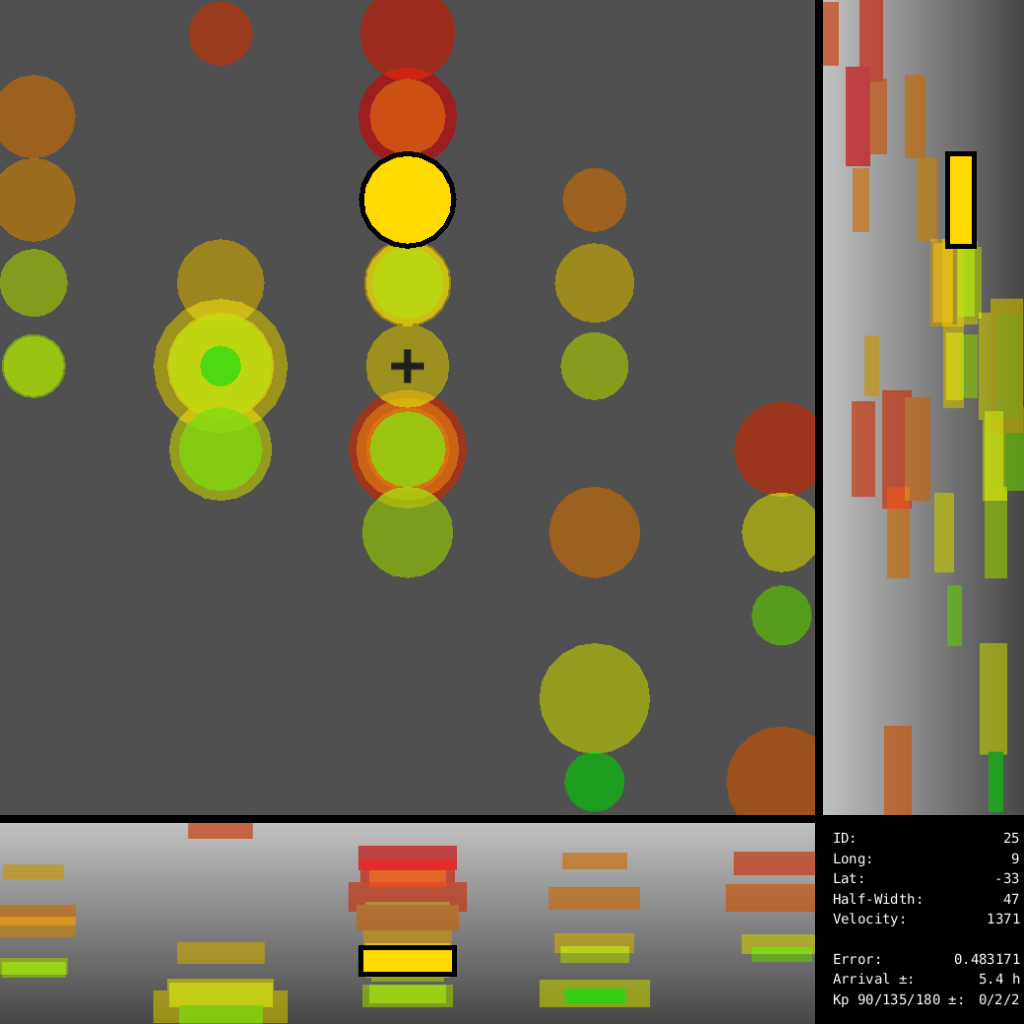
\includegraphics[height=\abImageHeight]{figures/EnsembleSelectionView.png}}
  }
%  \subfigure[Timeline View] {
%    \fbox{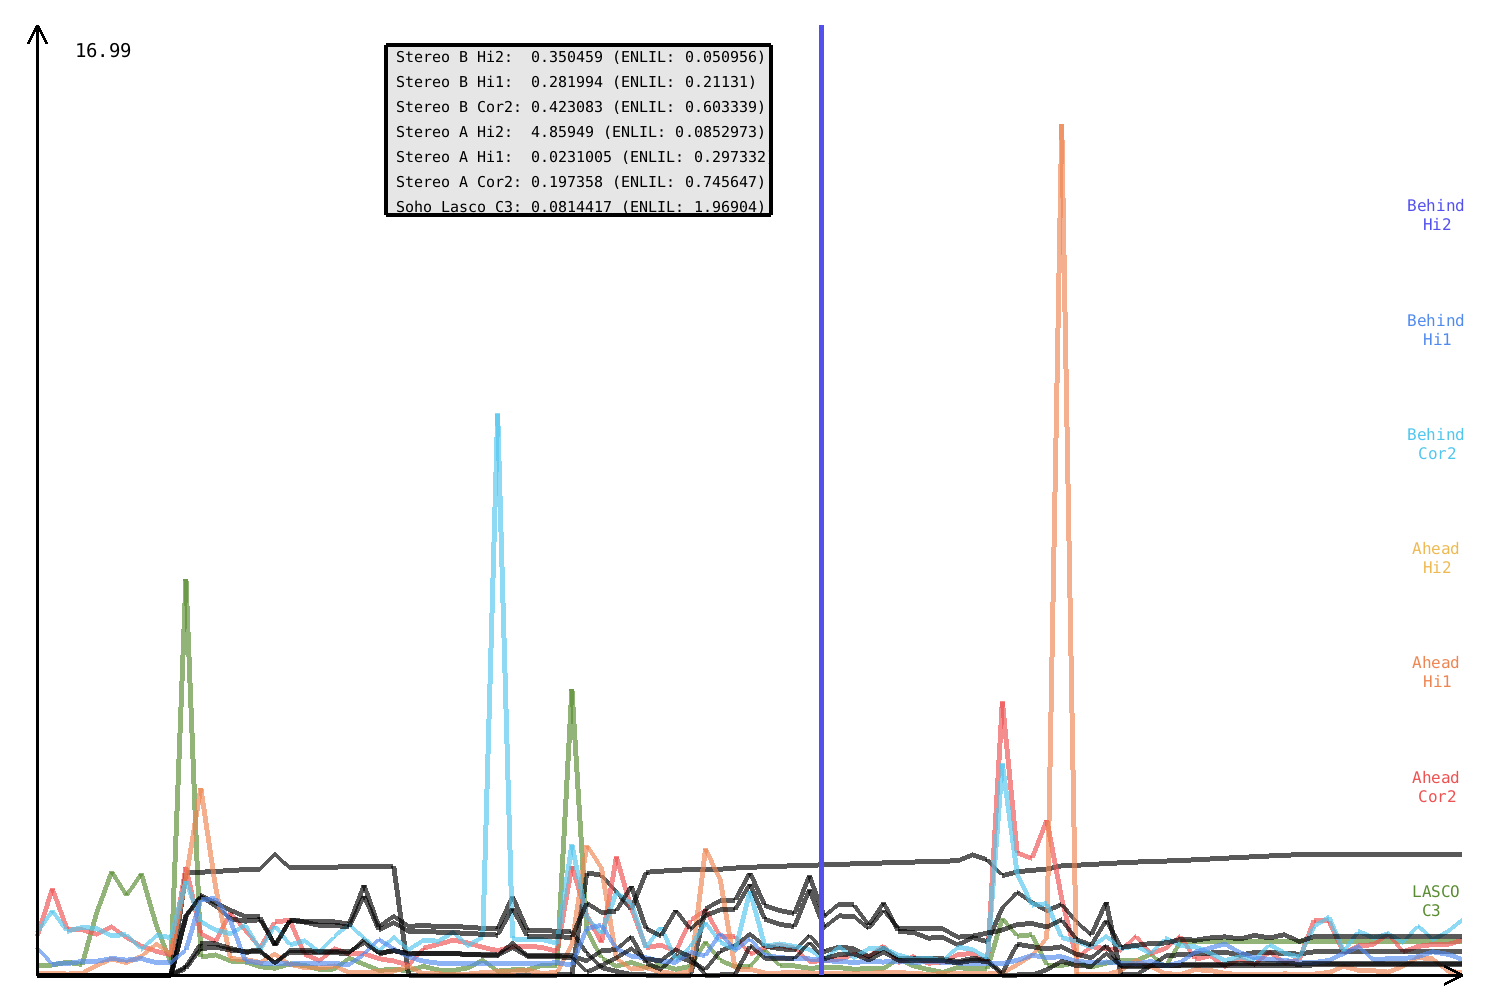
\includegraphics[height=\abImageHeight]{figures/TimelineView.png}}
%  }
  \subfigure[Spatial View] {
    \fbox{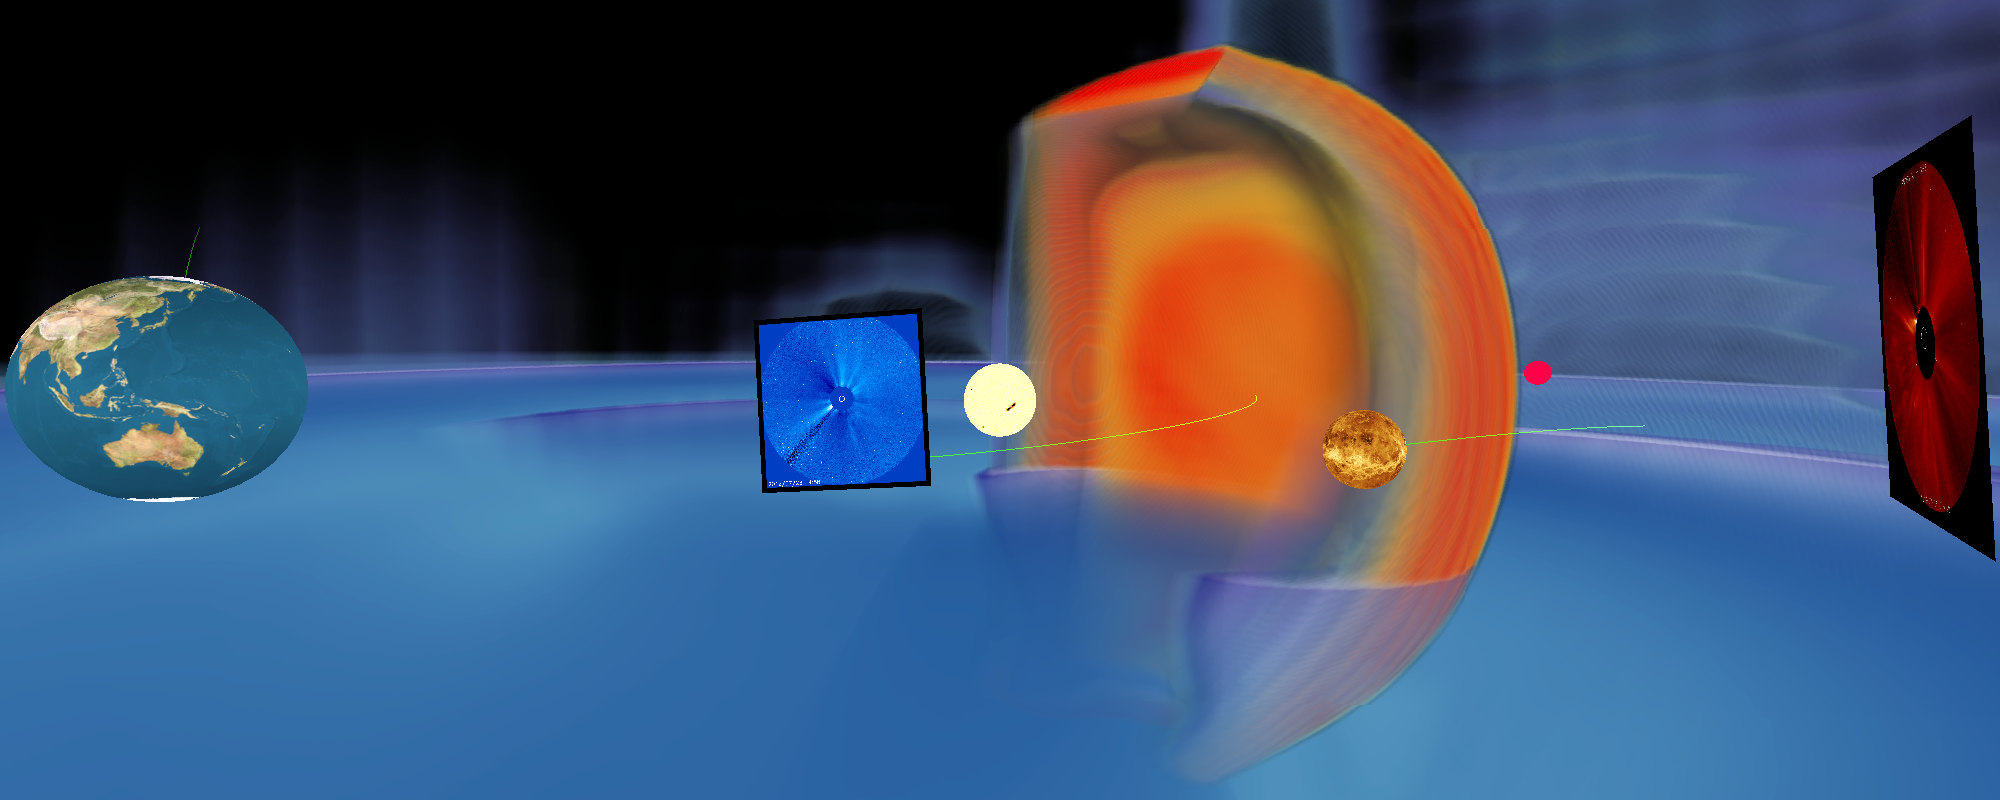
\includegraphics[height=\abImageHeight]{figures/teaser_rendering.png}}
  }
  \caption{Our proposed system helps space weather analysts to gain a better understanding of ensemble simulations of coronal mass ejections. The Ensemble Selection View (a) shows comparisons for all ensemble members with ground-truth, in-situ measurements to provide the user with a global overview. 
%The Timeline View (b) enables the comparison of time-dependent velocity data derived from optical flow analysis of satellite images and extracted velocity fields from the simulation for multiple instruments in the solar system.
The Spatial View (b) allows the inspection of an interactive volume rendering of the simulation data set, coregistered with satellite images, as well as spacecraft and planetary bodies.}
  \label{fig:teaser}
}

%% Uncomment below to disable the manuscript note
%\renewcommand{\manuscriptnotetxt}{}

%% Copyright space is enabled by default as required by guidelines.
%% It is disabled by the 'review' option or via the following command:
% \nocopyrightspace

%%%%%%%%%%%%%%%%%%%%%%%%%%%%%%%%%%%%%%%%%%%%%%%%%%%%%%%%%%%%%%%%
%%%%%%%%%%%%%%%%%%%%%% START OF THE PAPER %%%%%%%%%%%%%%%%%%%%%%
%%%%%%%%%%%%%%%%%%%%%%%%%%%%%%%%%%%%%%%%%%%%%%%%%%%%%%%%%%%%%%%%%

\newcommand{\kpIndex}{$\textrm{K}_\textrm{P}$}
\setlength\fboxsep{0pt}

\begin{document}
\firstsection{Introduction}
\maketitle
%% \section{Introduction} %for journal use above \firstsection{..} instead
\emph{Space weather} is the description of the environmental conditions in our solar system and their effects on planets, spacecraft, and human society. The effects influencing space weather in our solar system are created by the Sun. \emph{Coronal mass ejections} (CMEs) occur when magnetic field lines on the Sun's surface reconnect and plasma clouds are accelerated away from the Sun and into the solar system. An important part of \emph{Space weather forecasting} is the prediction of the direction and velocity of CMEs to forecast the arrival time and impact when they hit objects in the solar system, such as Earth or spacecraft. When spacecraft are hit by these events, they can cause irreparable damage to electronic systems. In the case of Earth, most of the plasma is deflected by Earth's magnetosphere and funneled towards the north and south pole, creating auroras. However, it also causes geomagnetically induced currents in terrestrial infrastructure, such as power grids. This happened in Quebec in 1989 when a CME struck Earth and induced currents in the power grid causing a blackout nine hours long. The biggest CME on record is the Carrington Event from 1859 that generated auroras as far south as the Sahara and induced currents in telegraph lines that gave electrical shocks to telegraph operators and sparked fires. The Lloyds insurance agency estimated that, in North America alone, a similar event today would cause up to \$2.6 trillion in damages and create blackouts of up to 2 years due to destroyed transformers~\cite{lloyds2013impact}. However, such a situation can be completely mitigated by accurate space weather forecasting.

Current CME predictions created by space weather agencies world-wide are based on magnetohydrodynamic simulations whose input parameters are derived from satellite imagery. In the state-of-the-art simulation code, the CME is modeled based on a cone originating from the Sun with a direction (\emph{longitude} and \emph{latitude}), \emph{speed}, and \emph{opening angle} as free parameters. Currently, these cone parameters are manually selected in satellite images using triangulation algorithms, which naturally introduces error into the simulation pipeline and thus requires verification. Providing a system for mitigating this uncertainty through visualization is the main contribution of this paper.

\begin{figure*}
\centering
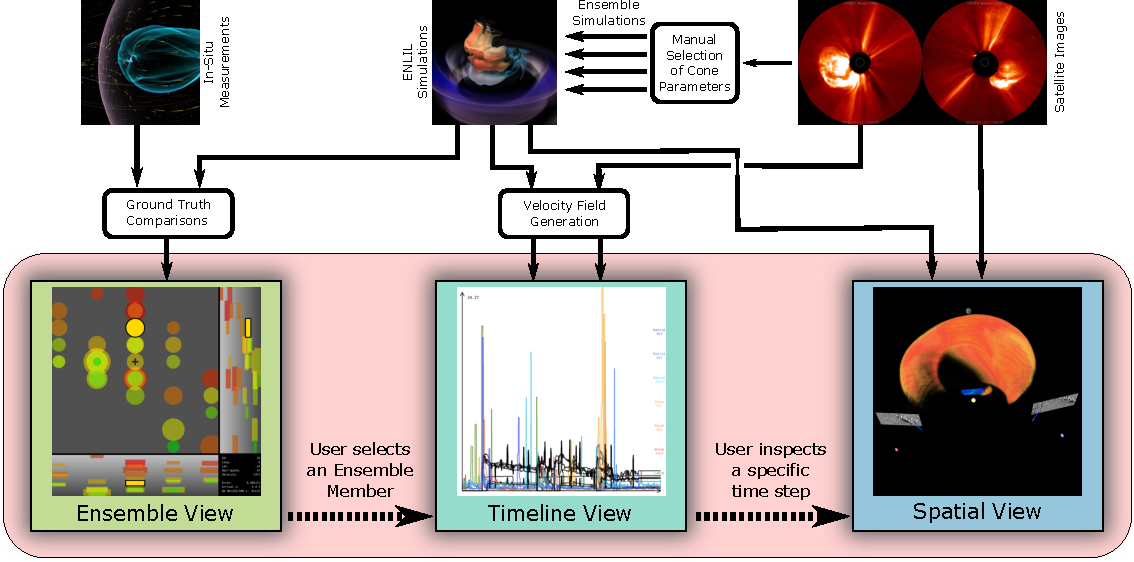
\includegraphics[width=\linewidth]{figures/workflow.pdf}
\caption{Our proposed three-step workflow for the analysis of CME ensemble runs and the data flow within our system. The available data (top) is preprocessed (middle) before being communicated through visualization (bottom). Using the views, the analyst starts with a global overview of all ensemble members (bottom left), and gains detailed information for specific members through use of the other views (bottom middle and right).}
\label{fig:workflow}
\end{figure*}

\begin{figure}[!b]
%\newcommand{\abImageWidth}{\columnwidth}
\centering
%\subfigure[The ENLIL simulation with Cone parameters]{
%  \fbox{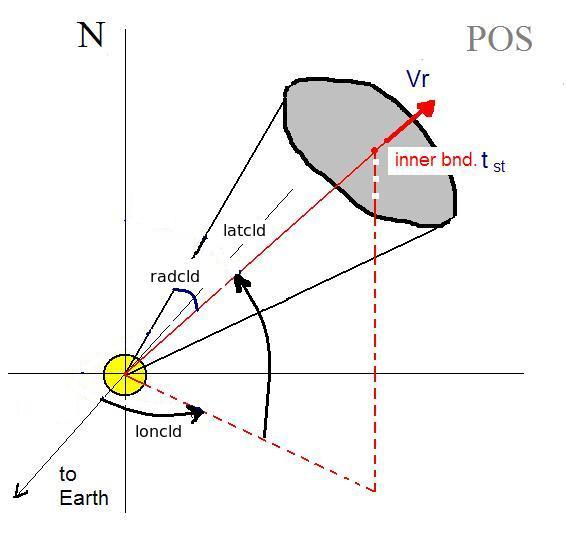
\includegraphics[width=\abImageWidth]{figures/Enlil.jpg}}
%    \label{fig:enlil}
%  }
%\hfill{}
%\subfigure[Coronagraph image of a coronal mass ejection with the Earth for scale]{
%\fbox{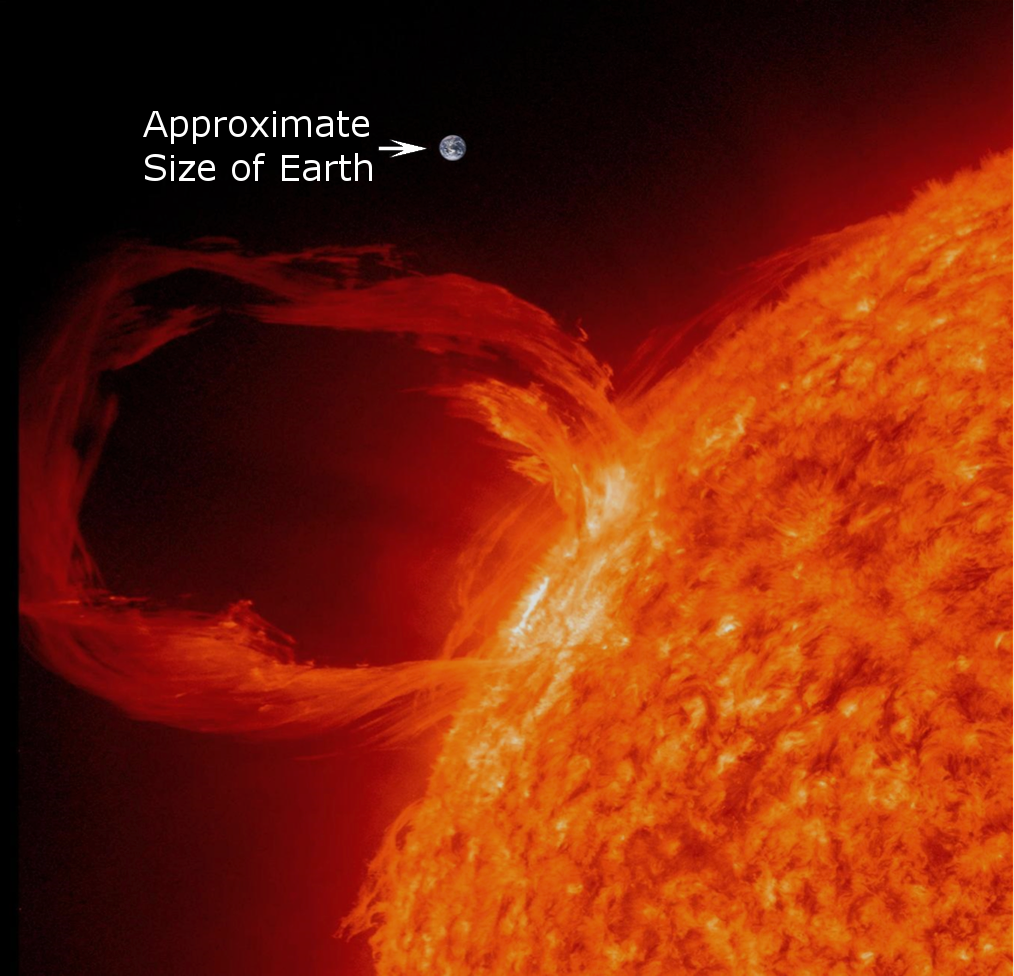
\includegraphics[width=\columnwidth]{figures/CME.png}}
\fbox{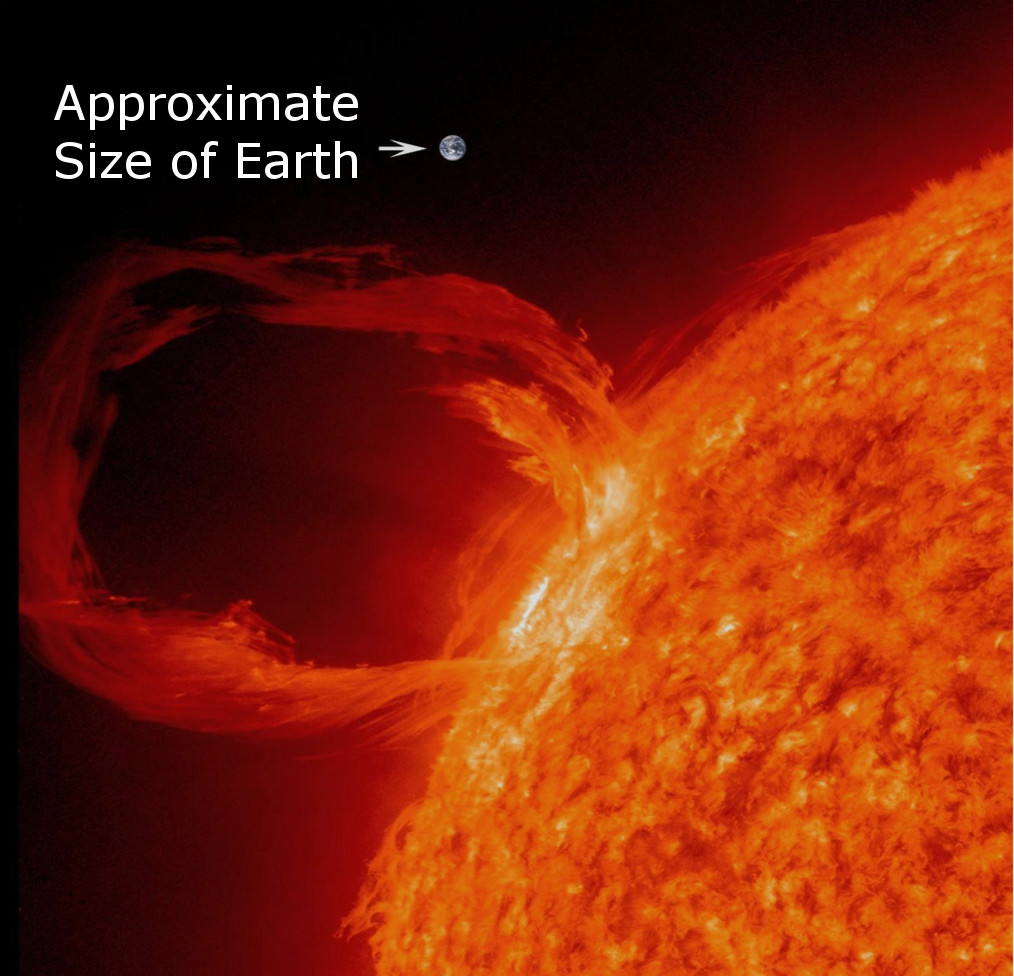
\includegraphics[width=0.5\columnwidth]{figures/CME.jpg}}
%}
\caption{Coronagraph image of an erupting coronal mass ejection with Earth shown to scale.}
\label{fig:cme}
\end{figure}

\section{Introducing a Visual CME Analysis Workflow}
To alleviate the impact of measurement inaccuracies, simulation ensembles are generated by varying the CME input parameters and performing simulations for each combination. Our visualization system uses a multi-view setup to provide space weather analysts with the tools to verify ensemble runs in two ways:

\begin{itemize}

\item{ground-truth measurements of the arrival time, speed, and geoeffectivity are measured and compared against the values predicted by each simulation.} 

\item{renderings of the simulation are compared with imagery from satellites to obtain time-varying information about the simulation's accuracy from multiple locations throughout the solar system.} 

\end{itemize}

A human-in-the-loop is needed for these verifications as the available data sources are noisy and uncertain. By providing an integrated and consistent system, we combine the different modalities and support the analyst in understanding the simulation results. It is currently not feasible to employ an automatic algorithm to determine whether a simulation accurately represents the measured reality due to the required expertise when dealing with, as of yet, not fully understood physical principles. 

Current systems used in simulation analysis do not integrate available data streams of ensemble members thus prohibiting the analyst from gaining deeper understanding of CMEs from them. In a participatory design phase together with analysts from one of the world-leading space weather research centers we have developed a novel three step visual workflow (see Figure~\ref{fig:workflow}) which provides the space weather analysts with a greater understanding of the influence of parameter values in the ensemble simulations: 

\begin{enumerate}

\item{\emph{glyph-based} visualization of ensambles providing access to the measured ground truth values. This allows for a quick reduction of the number of interesting ensemble members the analyst needs to inspect in detail. Furthermore, it allows the analyst to quickly see if any of the simulations match the ground truth data.}

\item{\emph{graph visualization} enabling inspection of the time-dependent measurements for each available satellite for a specific ensemble member. These measurements are generated by extracting the CME speed from simulations and comparing them with the speed derived by optical flow analysis of satellite images.}

\item{\emph{volumetric rendering} of the simulation results with integrated positions of different satellites, their instrument field of views, as well as planetary bodies. Our proposed system is the first to bring volumetric rendering and comparative time-dependent analysis into the space weather analysis workflow}

\end{enumerate} 

The result is a system that fuses multiple streams of data providing the space weather analyst with the means to inspect the details of ensemble simulations. As the physical processes governing the behavior of CMEs is not yet fully understood, visualization can have a beneficial impact in providing the space weather analysts with information to form and test new hypotheses to advance the field of solar physics.  

\section{Space Weather Simulation and Data Acquisition}
This section provides all necessary background information about space weather phenomena (Section~\ref{sec:spaceweather}), the satellites used for image data acquisition, the MHD simulations that are performed to acquire the volumetric data, the in-situ measurements that are used to verify the simulation runs (Section~\ref{sec:data}), and provides an overview of the currently employed workflow (Section~\ref{sec:currentworkflow}).

\subsection{Coronal Mass Ejections} \label{sec:spaceweather}
\begin{figure*}
\newcommand{\abAllCoronagraphImageHeight}{0.475\columnwidth}
\centering
\subfigure[STEREO A Cor2] {
  \fbox{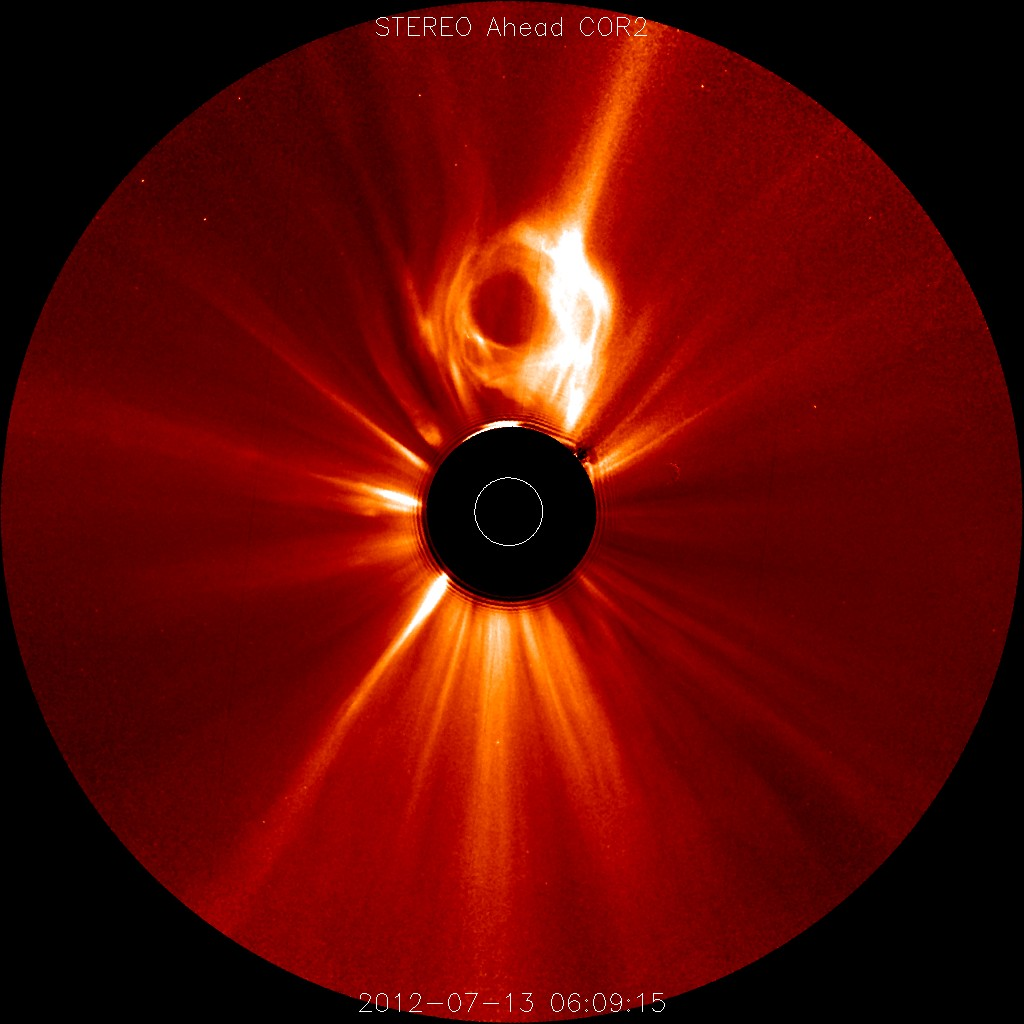
\includegraphics[width=\abAllCoronagraphImageHeight]{figures/20120713_060915_n4c2A.jpg}}
}
\subfigure[STEREO A HI 1 with Earth and the Milky Way in view] {
  \fbox{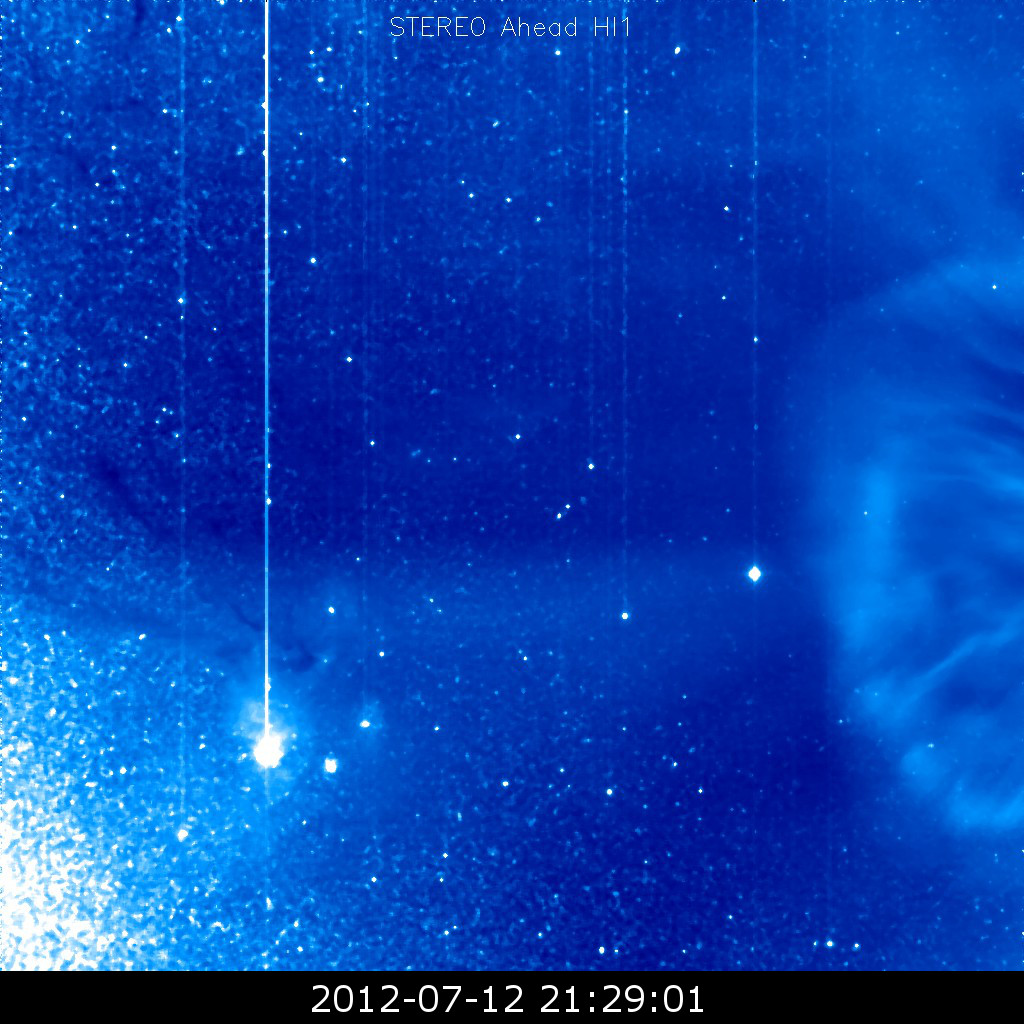
\includegraphics[width=\abAllCoronagraphImageHeight]{figures/20120712_212901_s4h1A.jpg}}
}
\subfigure[STEREO A HI 2 with the Milky Way in view] {
  \fbox{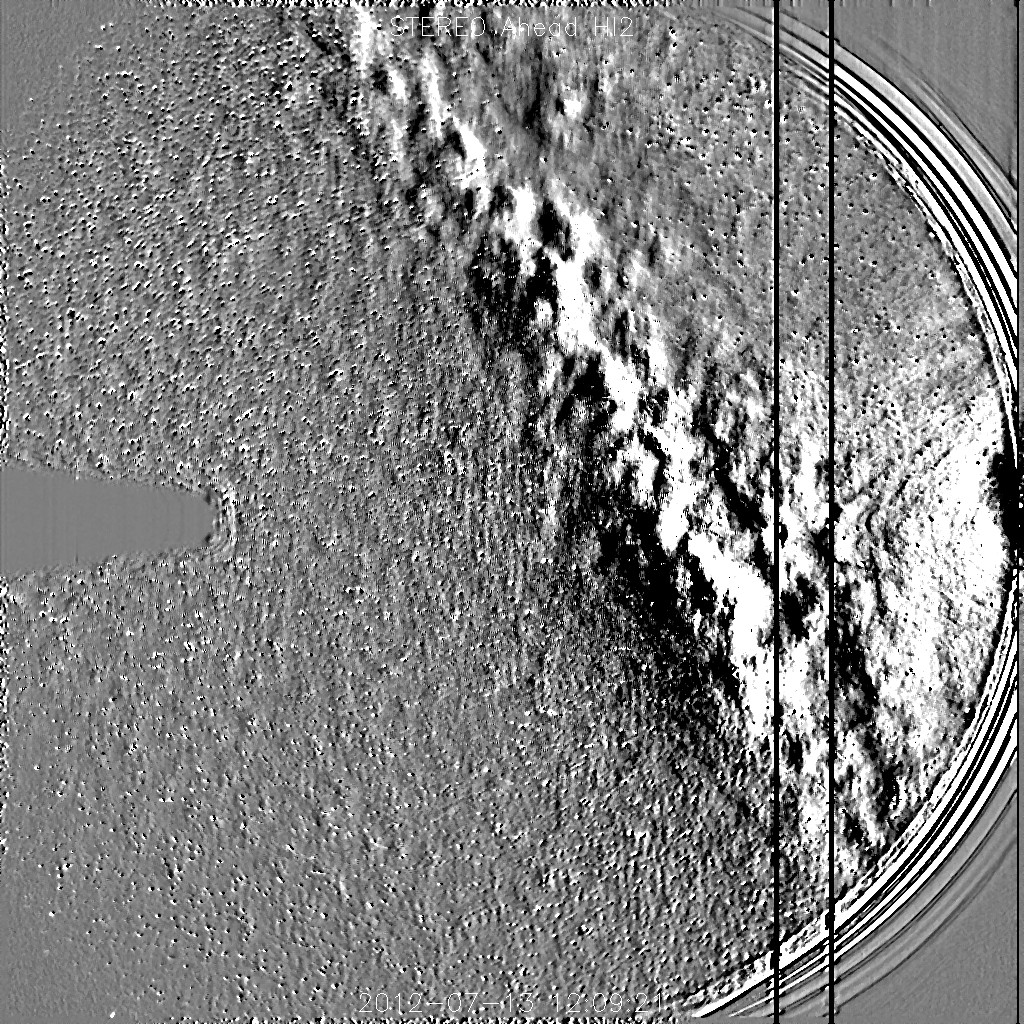
\includegraphics[width=\abAllCoronagraphImageHeight]{figures/20120713_120921_s4h2A.jpg}}
}
\subfigure[SOHO LASCO C3] {
  \fbox{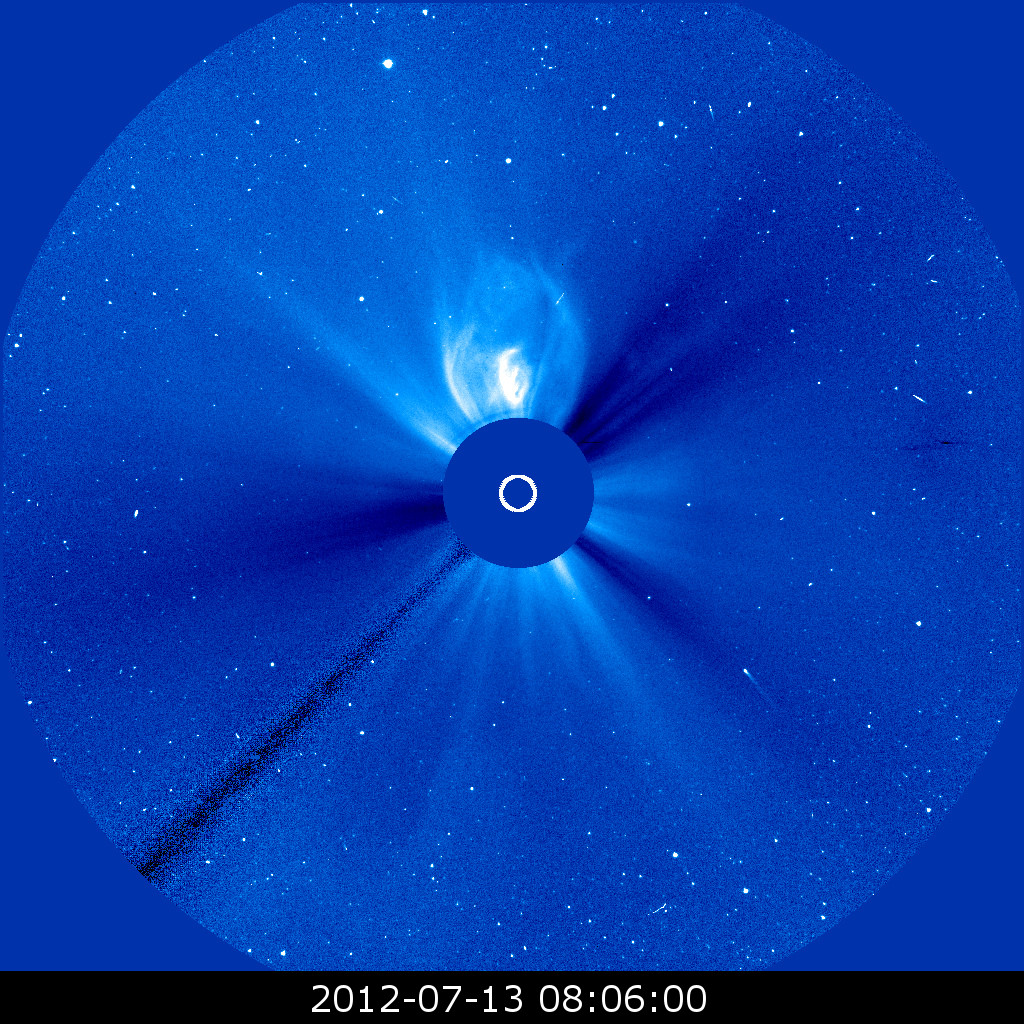
\includegraphics[width=\abAllCoronagraphImageHeight]{figures/20120713_0806_c3_1024.jpg}}
}
\caption{Images of four of the seven coronagraph imagers we use in our system. The Stereo A SECCHI suite of instruments (a), (b), and (c) gives a continuous view of the space between the Sun and Earth. Soho (d) views the Sun from Earth's perspective. The three missing images from STEREO B are similar to (a), (b), (c)}
\label{fig:coronagraph}
\end{figure*}


Space weather is a collective term that "describes the conditions in space that affect Earth and its technological systems. Space Weather is a consequence of the behavior of the Sun, the nature of Earth’s magnetic field and atmosphere, and our location in the solar system. The active elements of space weather are particles, electromagnetic energy, and magnetic fields [...]"~\cite{noaaprofile}.

One of the prominent elements of space weather are coronal mass ejections; large plasma clouds consisting of charged particles that are accelerated to speeds of 500--3000\,km/s~(see Figure~\ref{fig:cme}). They have been described as the "most energetic phenomena known to occur in the solar system"~\cite{Kahler:1987jt} and have a major impact on Earth and interplanetary space. Earth and its orbiting satellites are mostly protected by its magnetic field that deflects the stream of charged particles. However, a strong CME compresses Earth's magnetic field, exposing geostationary satellites to these high-intensity particles, thus increasing the likelihood of irreversible damage to satellites~\cite{Guhathakurta:2013cl}. Furthermore, the moving magnetic field induces currents on large, conductive structures on Earth, such as power grids, train tracks, or oil pipelines, which damages those infrastructures. Power lines are especially affected as connected transformers are sensitive to fluctuations and can be (and have been) damaged by the effects of a strong CME. An additional effect of a CME hitting Earth is an increase in radiation exposure to passengers of flights over the poles, furthermore increasing the necessity to predict these events to keep people from harm~\cite{Matthia:2009en}.

\subsection{Sensors and Simulation Data} \label{sec:data}
In our system, we use three sources of data. The first source is coronagraph images from three satellites in the solar system. These images provide the analyst with real-time information about the structure and time-evolution of the CME. The second source of data is magnetohydrodynamics (MHD) simulations of the CME that produces a time-varying, multivariate dataset of the solar system. The simulations are initialized by the satellite images and are used to predict the arrival time and strength at various targets. The third source is ground-truth in-situ measurements from spacecraft or ground stations that are used to verify and refine the MHD simulations for increased prediction accuracy for future CMEs. Figure~\ref{fig:workflow} presents the data flow in our visualization system.

\subsubsection{Coronagraphs} \label{sec:coronagraph}
\begin{figure}[b!]
\newcommand{\abImageWidth}{0.465\columnwidth}
\centering
\subfigure[Orbits of SOHO, STEREO A, and STEREO B in the solar system] {
  \fbox{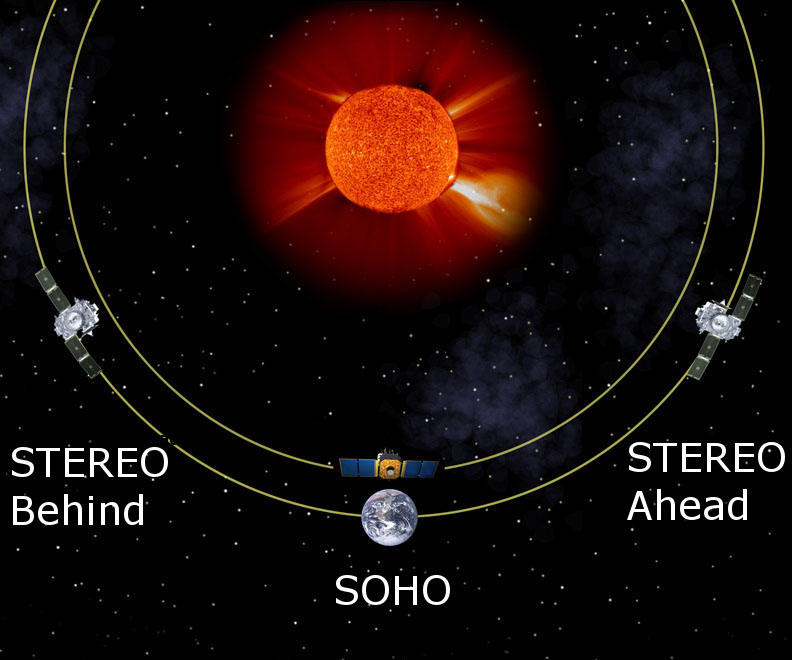
\includegraphics[width=\abImageWidth]{figures/ST_orbit_Nov09_v3.jpg}}
  \label{fig:spacecraftlocation}
}
\hfill{}
\subfigure[The Stereo B SECCHI suite of coronagraphs, Cor2, HI 1, and HI 2] {
  \fbox{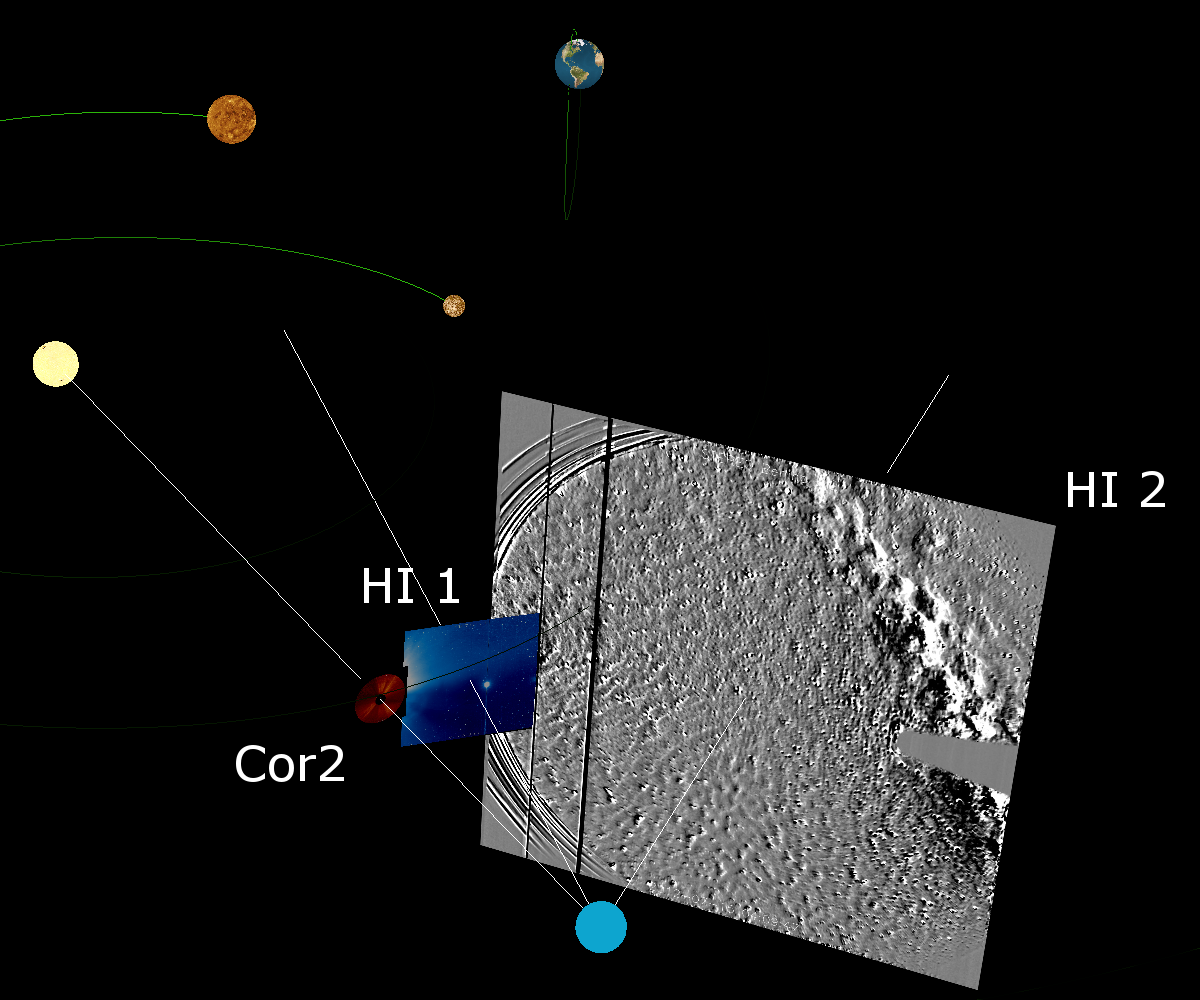
\includegraphics[width=\abImageWidth]{figures/secchi_labels.png}}
  \label{fig:coronagraphgallery}
}
\caption{(a) The orbits and locations of SOHO, STEREO A and B in November 2009. (b) The location and orientations of the three coronagraph imagers of STEREO B with Mercury, Venus, Earth, and the Sun in the same view (not to scale). The layout of the images for STEREO A are mirrored horizontally.}
\end{figure}

Coronagraphs are optical telescopes pointed at the Sun that block out the solar surface with a physical disc in order to capture the much fainter surrounding corona (see Figure~\ref{fig:coronagraph}). In our system, we utilize coronagraph images from three satellites: SOHO and the identical satellites STEREO A and STEREO B. Including more observatories would not be beneficial, as they would be located on the Earth and thus have the same viewpoint as SOHO~(see Figure~\ref{fig:spacecraftlocation}). Coronagraphs provide the space weather analyst with the data to study the time-evolution and internal structure of CMEs.

\noindent {\bfseries SOHO.} The Solar and Heliospheric Observatory (SOHO) is a satellite orbiting around the L$_1$ Lagrangian point, constantly pointing at and allowing for an uninterrupted observation of the Sun with the Large Angle and Spectrometric Coronagraph (LASCO), which contains multiple coronagraphs~\cite{Brueckner:1995cb}. We are utilizing the C3 coronagraph that shows the area from 3.7 to 32 solar radii with a field of view of 8 degrees. SOHO produces one image every 12 minutes. 

%In preprocessing, the images are aligned to solar north and any additional roll angle is extracted from the meta data and applied to the image~\cite{wells1981fits}.

\noindent {\bfseries STEREO.} The Solar Terrestrial Relations Observatory is a set of two identical satellites, STEREO A and STEREO B, that orbit the Sun. A's orbit is slightly lower than Earth's, while B's orbit is slightly higher. Thus, from Earth's point of view, A is moving ahead of Earth while B is falling behind. The separation between A and B allows for stereoscopic images and thus 3-dimensional reconstruction of CMEs. We make use of three coronagraphs~\cite{Socker:2000ic}: COR2 observes the Sun from 2.5--15 solar radii with a field of view of 8\degree\ and provides an image every 15 minutes. The HI1 and HI2 imagers observe the space between the Sun and Earth from 15--90 solar radii (20\degree\ field of view) and 70--330 solar radii (70\degree\ field of view) with cadences of 40 minutes and 2 hours respectively. Figure~\ref{fig:coronagraphgallery} shows the respective fields of view of the three instruments side-by-side.

\subsubsection{Magnetohydrodynamics Simulation} \label{sec:mhd}
In our system, we use the state-of-the-art multivariate MHD simulation code ENLIL for simulating the CME~\cite{odstrcil2002merging}. Figure~\ref{fig:teaser} (right) shows the results of the rendering of one time step. The variables of the simulation that we are using in our system are the location, the velocity, particle density, and a tracer particle for discriminating the CME. The ENLIL simulations are performed on a spherical grid. The state-of-the-art method of performing CME simulations is to assume that the CME input parameteres are approximated by a cone~\cite{Arge:2000jz}, described by four parameters: location in longitude and latitude, speed, and the opening angle. These are manually determined using a tool called Stereo CAT, that uses triangulation on STEREO A and STEREO B observations~\cite{Millward:2013cm}.%The manual process of selecting a leading edge and opening angle naturally introduces inaccuracies in the simulation.

%Furthermore, while the assumption of a conical shape for the erupting CME is still state-of-the-art, it is known that this shape does not accurately reflect the shape of the CME in all cases, leading to a further requirement of analysis tools.

%These can be directly measured with instruments onboard the spacecraft and have been used in the past to study the structure of a passing CME.
\subsubsection{Ground Truth Measurements} \label{sec:insitu}
Two direct in-situ measurements are the CME's arrival time and speed at Earth or a spacecraft. These ground truth measurements are the main focus of the space weather forecasting. Another measurement is the geoeffectivity index \kpIndex. It is a measure of general planetary-wide geomagnetic disturbances that uses a quasi-logarithmic scale from 0 to 9. Predicting this information is important as it is a direct measure of the strength of the CME's effect on earth. However, ENLIL does not model the direction of the CME's internal magnetic field that influences the \kpIndex . Therefore, three angle scenarios of 90\degree , 135\degree , and 180\degree\ are assumed for the interplanetary magnetic field, thus providing an estimate of possible maximum values. The comparison must be made between the measured geoeffectivity and all three simulated geoeffectivities. Comparing the predicted values with the measured values for previous CMEs provides the scientists with valuable insight for space weather forecasting.

\subsection{Current Tools} \label{sec:currentworkflow}
\begin{figure}
\newcommand{\abImageWidth}{\columnwidth}
\centering
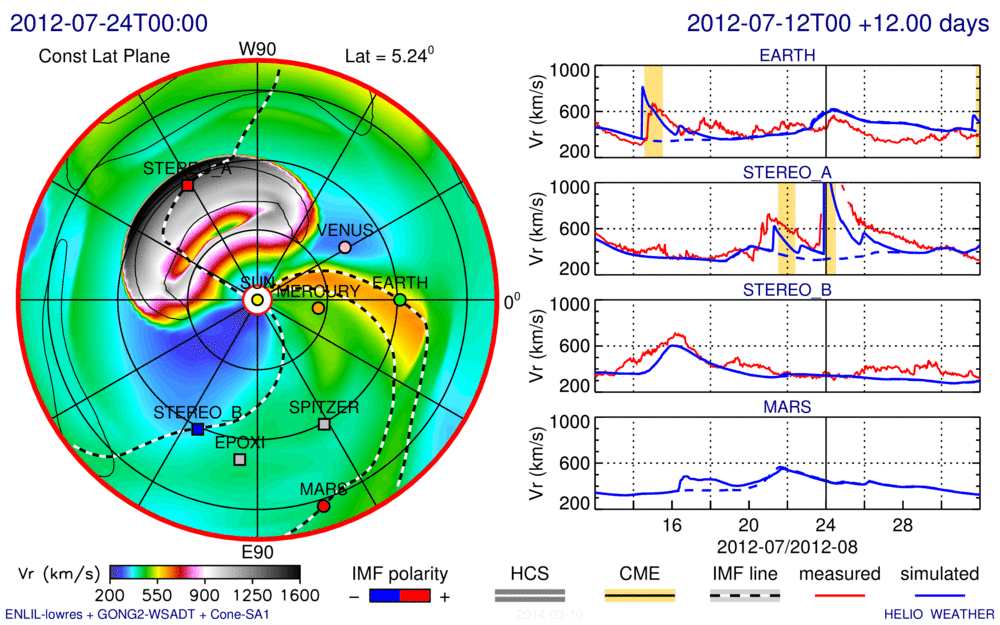
\includegraphics[width=\abImageWidth]{figures/current_workflow.png}
\caption{The currently employed workflow when analyzing single simulations of coronal mass ejections. The plot does not convey the 3 dimensional structure of the CME.}
\label{fig:currentworkflow:single}
\end{figure}

The tools currently available to the space weather analysts are fairly limited. Figure~\ref{fig:currentworkflow:single} shows the current analysis tool used for a single CME simulation. The available plots do not provide any information about the CME's three dimensional movement and show the comparison of the radial velocity only at predetermined locations. A major requirement from the analysts was to be able to view the full 3 dimensional data to be able to see internal structures of CMEs that are hidden in the available 2 dimensional slices.

Furthermore, the current tools do not translate well when dealing with multiple simulation ensembles. Figure~\ref{fig:currentworkflow:ensemble} shows one of many plots that are generated for the important measurements. There is no rendering of the CME ensembles, but only the representation of each ensemble run in the available plots without linked views or a mental registration between the plots. In order for the analyst to gain information about a specific ensemble member, multiple plots have to be manually registered before a comparison is made. This limitation is the reason that, currently, only a statistical analysis, rather than a detailed analysis, of the ensemble runs are made~\cite{mays2015ensemble}. While this statistical analysis produces information about the quality of the ensemble, it does not allow for detailed inspection of individual ensemble members to help understanding why ensemble members are not correct or gain additional information about individual ensemble members. We deal with this deficiency in our proposed system.

\begin{figure}
\newcommand{\abImageWidth}{\columnwidth}
\centering
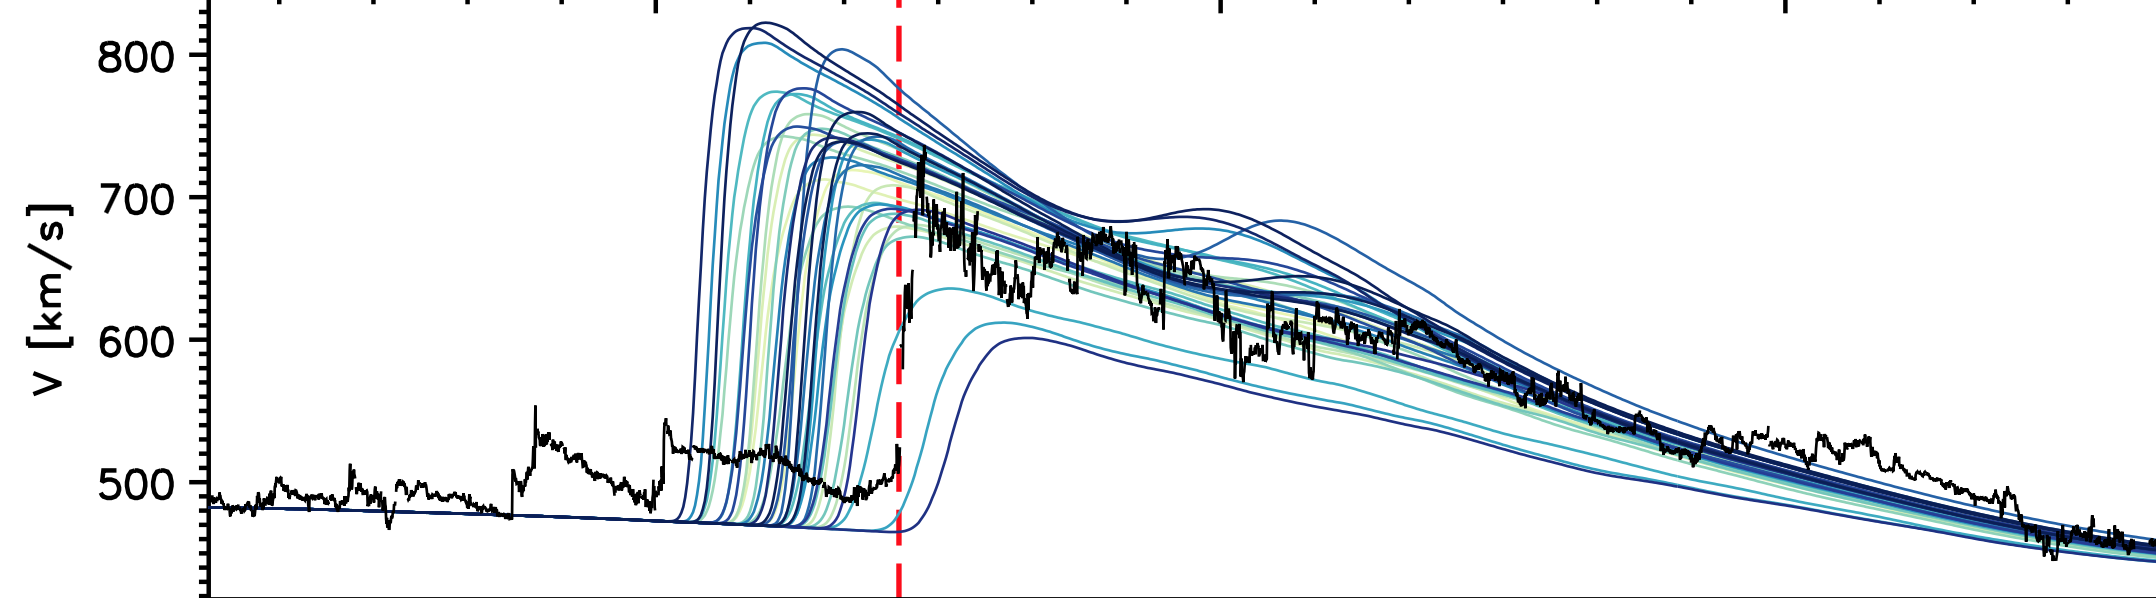
\includegraphics[width=\abImageWidth]{figures/current_workflow_ensemble.png}
\caption{One of the views in the current workflow used to analyze ensemble simulations. The spread of the simulations is shown for a single location with no mental registration to other locations.}
\label{fig:currentworkflow:ensemble}
\end{figure}

\section{Related Work}
\noindent {\bfseries Ensemble visualization.} Notable work dealing with the visualization of ensembles was done by Bruckner and M\"oller, who developed a system to allow the user to explore a simulation parameter space in order to incrementally reach a desired result~\cite{bruckner2010result}. One of the differences to our framework is the a priori unknown desired result. Naturally, many similarities exist with the field of weather forecasting on Earth, which has greatly matured over the years. Sanyal~\etal\ developed a system to explore ensemble simulations for weather forecasting that is most similar to ours~\cite{sanyal2010noodles}. However, the inherent differences in weather forecasting compared to space weather forecasting (2.5D structures vs. full 3D structures, the limited amount of measurement points, and missing theoretical frameworks) limit the applicability of their approach to space weather. Potter~\etal\ presented a system that uses a multi-view setup for ensemble visualization of statistics in climate modeling~\cite{potter2009ensemble}. Their approach informed our choice for a system based on a multi-view setup. There exist a plethora of ensemble visualization techniques that work well on 2 dimensional data, but unfortunately fail to do so in our case. Alabi~\etal\ use a surface slicing approach to show ensemble geometries at once and provide insight into multiple ensemble runs at once~\cite{alabi2012comparative}. This technique is not applicable in our case as we deal with volumetric renderings without a clear geometric representation. Whitaker~\etal\ generalized contour boxplots to handle ensemble data and aggregate their representations~\cite{whitaker2013contour}, while Kopp~\etal\ are using heatmaps to show the distribution of ensemble members~\cite{kopp2014decision}. In both cases, however, the technique is difficult to generalize in three dimensions and thus not usable in our system.

\noindent {\bfseries Space weather.} One of the first attempts of rendering CME simulations was performed by Wang~\etal\ on specialized hardware, allowing for interactive frame rates~\cite{wang2004visualization}. The validity of time-dependent comparisons of CME simulations with satellite imagery was shown in related work by Manchester~\etal ~\cite{manchester2008three} and Rusin~\etal ~\cite{rusin2010comparing}, while Lugaz analyzed the expected accuracy and possible sources of error in this method~\cite{lugaz2010accuracy}. Many visualization techniques have been applied to coronagraph images and coronal mass ejections. Jackson~\etal\ reconstructed a three dimensional volume from SMEI's white-light observations and compared these to coronagraph images. Colaninno and Vourlidas proved in principle that the application of optical flow analysis to coronagraph images of CMEs is feasible. They found that "optical flow maps can [...] provide quantitative measurements"~\cite{Colaninno:2006ef}. Thernisien~\etal\ analyzed the effectiveness of using the STEREO satellites to do CME prediction~\cite{Thernisien:2009hx}, as well as comparing the predictive powers between pre-STEREO and STEREO images~\cite{Thernisien:2011fl}. M\"ostl \etal\ performed a similar evaluation on 22 CMEs using the STEREO's HI instrument suite.~\cite{Mostl:2014iv}. Pulkkinen~\etal\ described a method that automatically generates cone parameters from LASCO images by image filtering~\cite{Pulkkinen:2009gb}. Millward~\etal\ designed the software that allows the space weather analysts to manually segment the CME in multiple time steps from multiple view points in order to derive the necessary simulation boundary conditions~\cite{Millward:2013cm}. They also performed an evaluation, achieving a mean CME arrival time forecast accuracy of 7.5h. A variation of this method is currently applied to generate the parameters for the ensemble simulation



%\subsubsection{STEREO}
%Cor2: white light Lyot coronagraph (2.5 - 15 solar radii); orientation: top $\rightarrow$ Solar North; 8 degrees opening angle; isoscele triangle: $a = \frac{2h}{\tan \theta}$
%HI1: 20 degrees FoV; 14.0 degrees off-point; (15-90 solar radii); cadence: 40 minutes; orientation: top $\rightarrow$ equatorial North
%HI2: 70 degrees FoV; 53.7 degrees off-point (70-330 solar radii); cadence: 2 hr; mean square error in positioning (HI2-A: 0.78 pixel, HI2-B: 1.48 pixel; firstHI\_Instrument\_Paper\_Revised  ; self-calibrating since images are used as star trackers; orientation: top $\rightarrow$ equatorial North; not properly usable due to Thomson effect \cite{howard2012thomson, deforest2013thomson, howard2013thomson, vourlidas2006proper, minnaert1930continuous, lugaz2008brightness}; experts want to see it included nevertheless. A CME itself is an optially thin medium which interacts with the Sun's visible light through Thomson scattering~\cite{}. More research has to be done on this end. This is the reason we don't do image comparisons.
%Overlap between HI1 and HI2 of about 5 degrees

%\subsection{MHD Simulations}
%\begin{itemize}
%\item What is ENLIL \cite{odstrcil2002merging}
%\item HEEQ coordinate system; cf. orbit of planets (prograde vs retrograde)
%\item Explain SOTA (cone-model) of boundary conditions
%\item Cone model is a very broad approximation of actual shape of the CME (Example: big flare that missed Earth $\rightarrow$ assumptions wrong)
%\item Sun's rotation causes CME to spiral
%\end{itemize}

\section{System}
Together with domain experts, we have developed a system that is based on a three-tier workflow (see Figure~\ref{fig:workflow}) to provide the space weather analysts with a greater understanding of the influence of parameter values in ensemble simulations. The parameter sensitivity in these simulations is currently not well understood, as ensemble simulation techniques have only recently been integrated into the analyst's toolbox. By creating a visualization system that provides the tools to browse, inspect, and understand the effect of parameter values on the simulation runs, we support the scientific discoveries to bringing ensemble simulations in operational forecasting, thus improving the forecasting capabilities.

For each ensemble member, a glyph-based comparison with in-situ measurements is presented in the \emph{Ensemble Selection View} (Section~\ref{sec:selection}, Figure~\ref{fig:selection}). In this view the comparisons to the ground truth data for all simulations are available at one glance. This allows the analyst to quickly gain an overview of the ensemble and make visual correlation between the input parameters and the prediction accuracy. The time-varying information of image-based comparisons between simulation and satellite imagery is shown in the \emph{Timeline View} (Section~\ref{sec:timeline}, Figure~\ref{fig:timeline}). This view shows, for a specific ensemble member, the speeds derived from an optical flow analysis and the simulated speed, thus providing the analyst with insight of time-of-flight velocity changes. This enables the analyst to quickly assess at which time a simulation error manifested. Each time step in the Timeline View can be selected and inspected in the \emph{Spatial View} (Section~\ref{sec:rendering}, Figure~\ref{fig:rendering}). This view shows the volume rendering of the CME simulation coregistered with the available satellite images at their correct positions and locations of spacecraft and planets. This view allows the analyst to inspect the 3 dimensional structure of the CME. This feature that was not available in the current workflow, but that has been requested by the analysts. The comparison of the rendering result with the satellite images is further used to inspect and gain insight about the structure of the CME.

%The proposed workflow for the analyst is to inspect the Ensemble Selection View first, getting an overview of the accuracy and validity of ensemble members. Afterwards, the Timeline View is utilized for a subset of interesting ensemble members to gain a deeper understanding of the time-dependent comparisons, grouped by satellites and instruments. Finally, the Spatial View is used to inspect the specific time steps that were used for the comparison by viewing the volumetric rendering of the CME embedded with the satellite images, spacecraft, and planetary bodies. Using this approach, the expert gains a quick overview and can inspect a lot of information about the ensemble runs in a short time.

\subsection{Ensemble Selection View} \label{sec:selection}
\begin{figure}
\newcommand{\abEnsembleImageHeight}{0.9\columnwidth}
\centering
\fbox{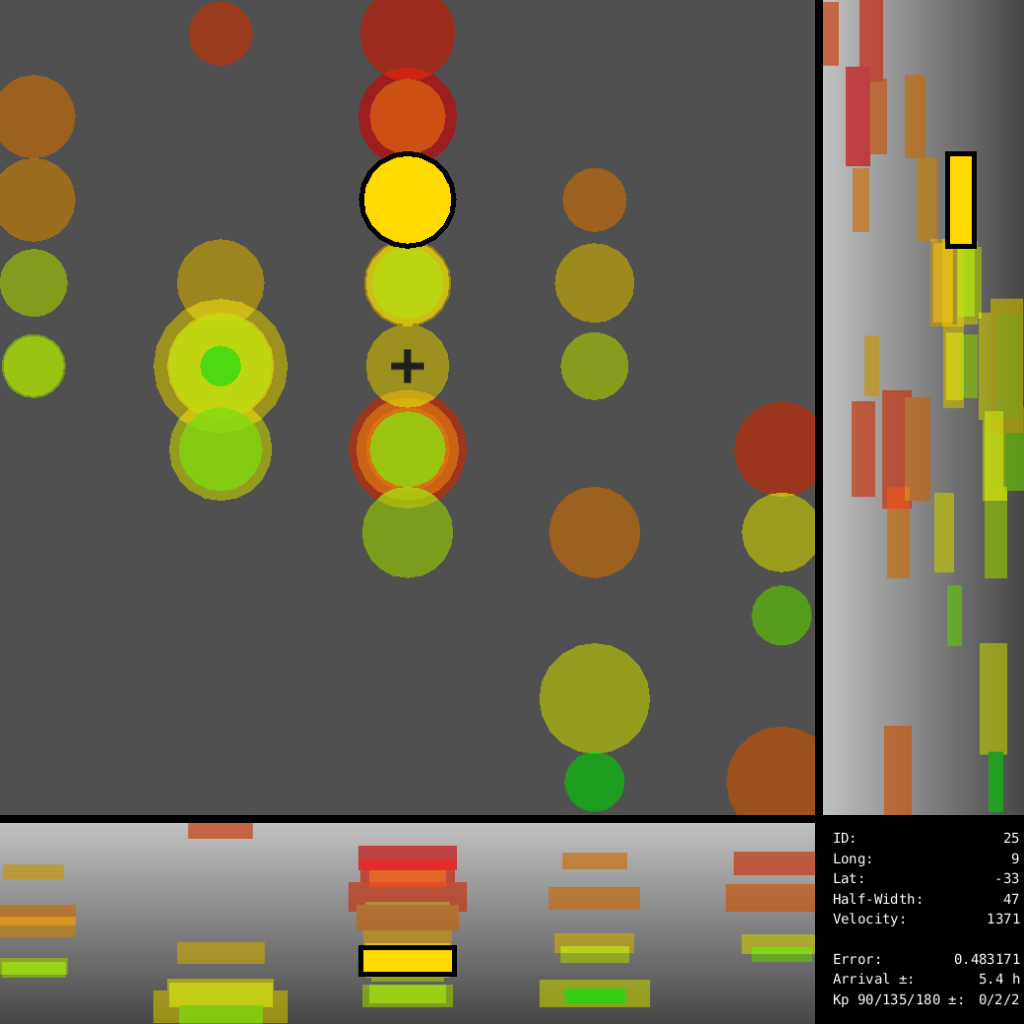
\includegraphics[width=\abEnsembleImageHeight]{figures/EnsembleSelectionView.png}}
\caption{The Ensemble Selection view provides an overview of all ensemble member and their comparisons to ground truth, in-situ measurements such as arrival time, speed, and geoeffectivity. Each ensemble is represented by a glyph and located according to the 4 dimensional input parameters.}
\label{fig:selection}
\end{figure}

\begin{figure}
\newcommand{\abImageWidth}{0.9\columnwidth}
\centering
\fbox{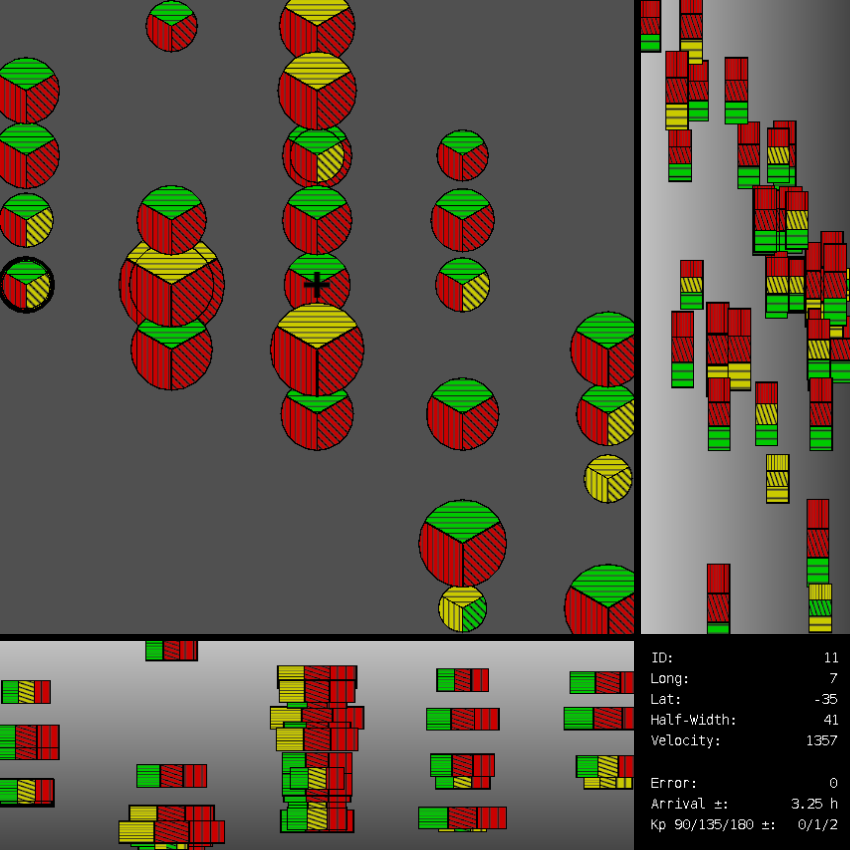
\includegraphics[width=\abImageWidth]{figures/ensemble_kp.png}}
\caption{The Ensemble Selection View showing the \kpIndex\ indices for all ensemble runs. The transparent lines agree with the orientation of the magnetic clock angle of 90\degree\ (=horizontal), 135\degree\ (=angled), and 180\degree\ (=vertical) for all ensemble members.}
\label{fig:selectionkp}
\end{figure}

\begin{figure*}
%\newcommand{\abImageWidth}{1.4\columnwidth}
%\newcommand{\abSmallImageWidth}{0.\columnwidth}
\newcommand{\abImageHeight}{5.25cm}
\centering
\subfigure {
  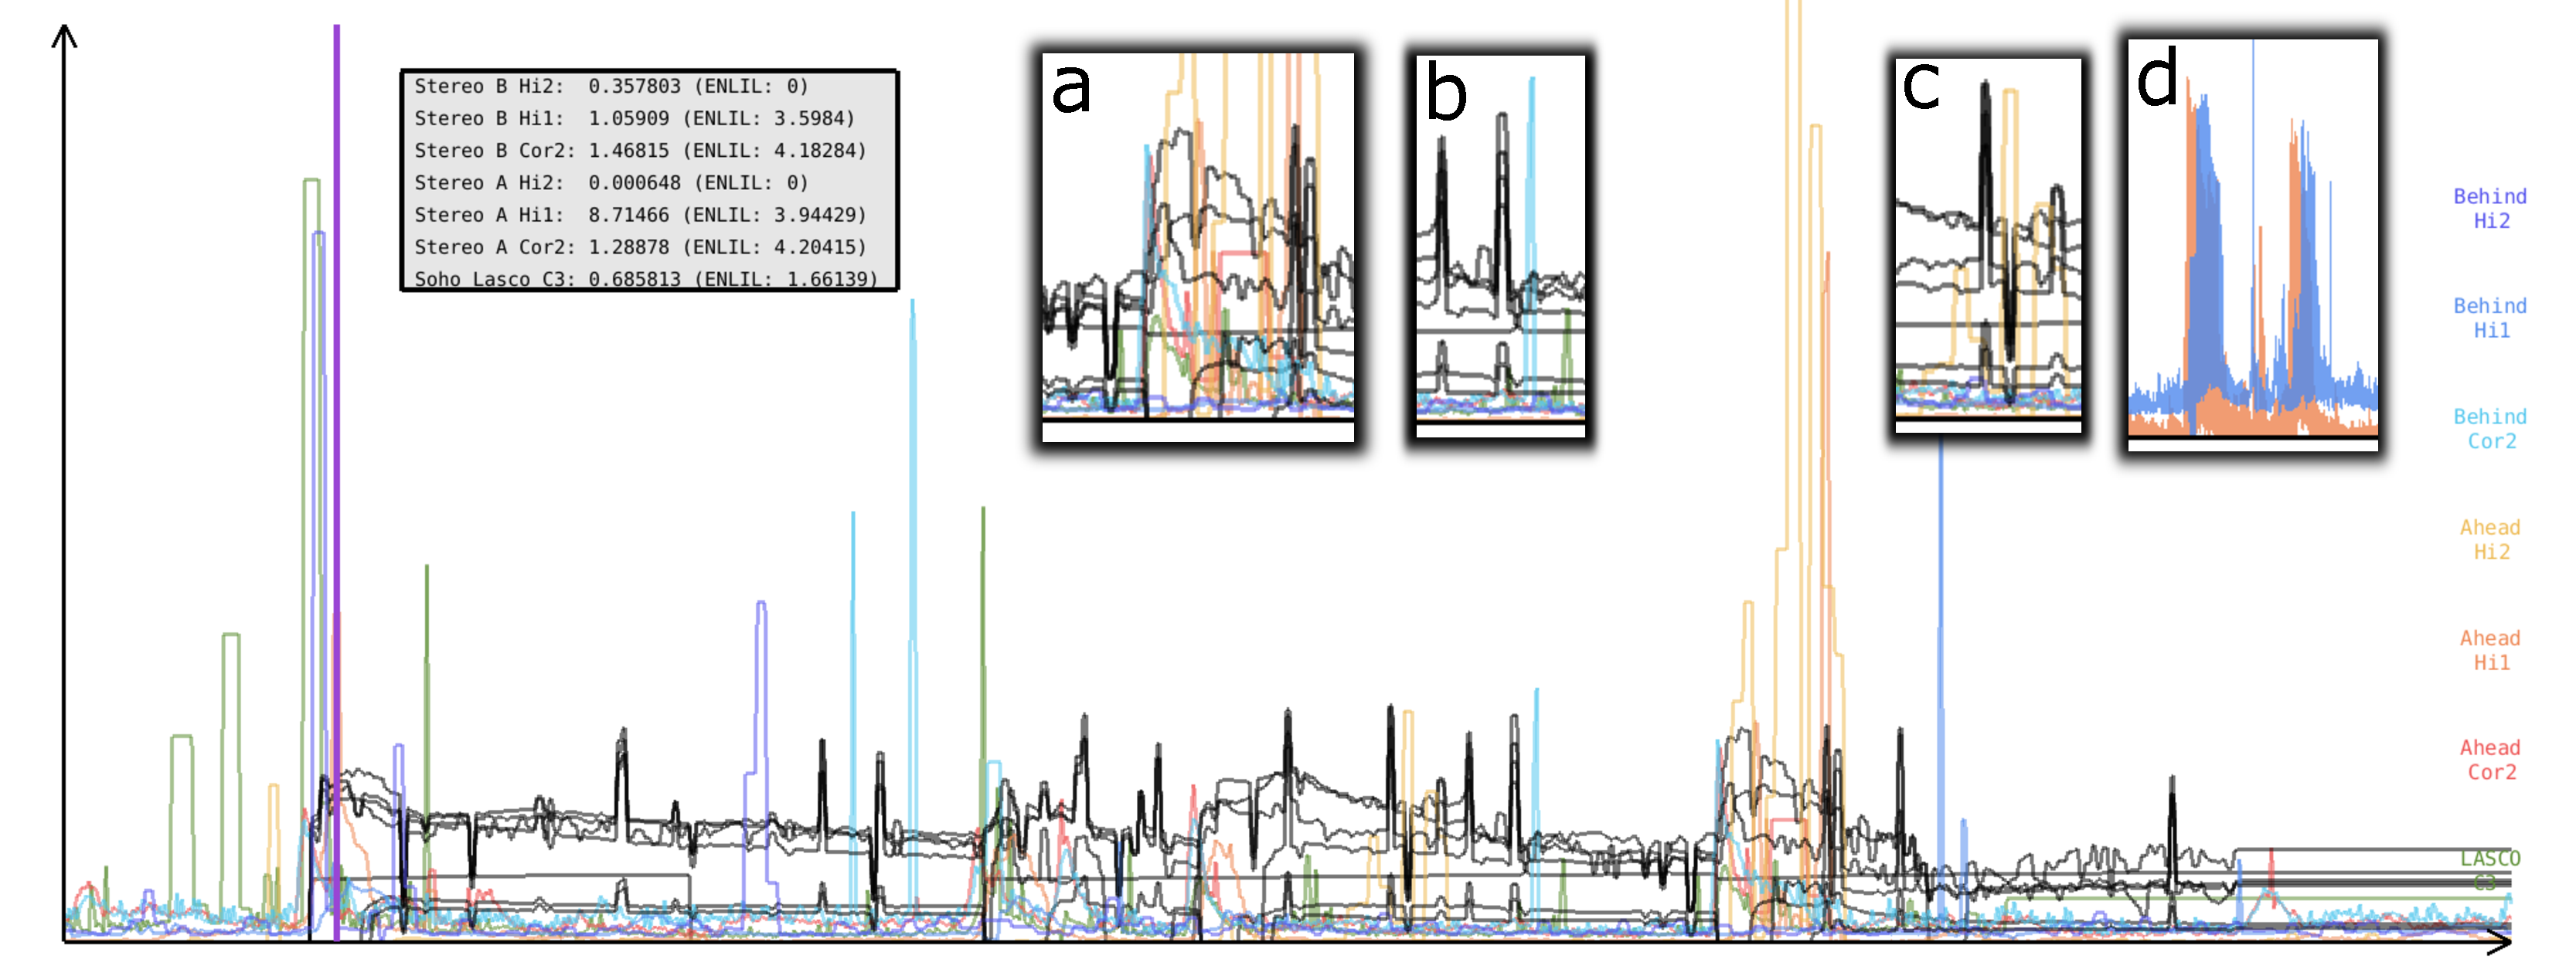
\includegraphics[height=\abImageHeight]{figures/timeline.pdf}
}
%  \subfigure {
%    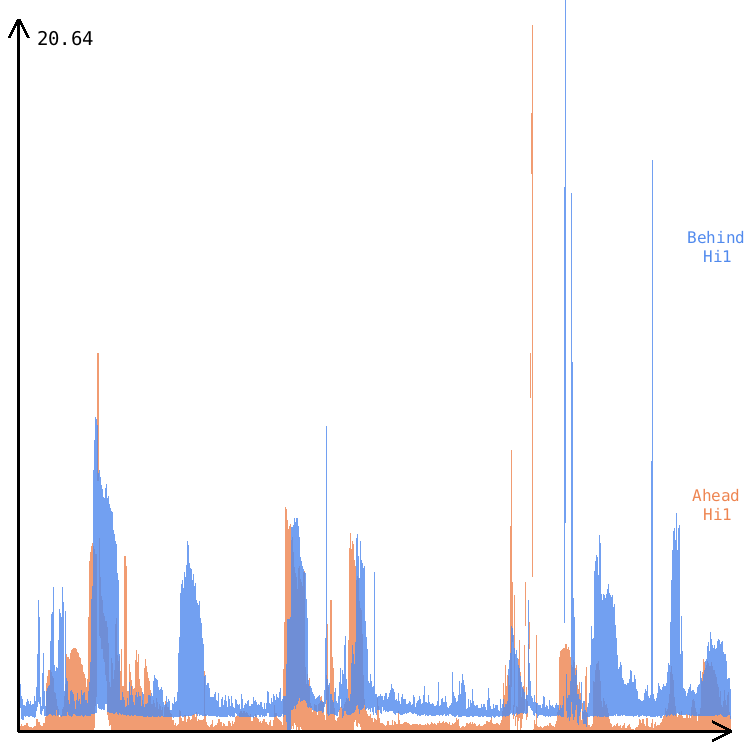
\includegraphics[width=\abSmallImageWidth]{figures/timelineview_hi1.png}
%  }
%  \subfigure {
%    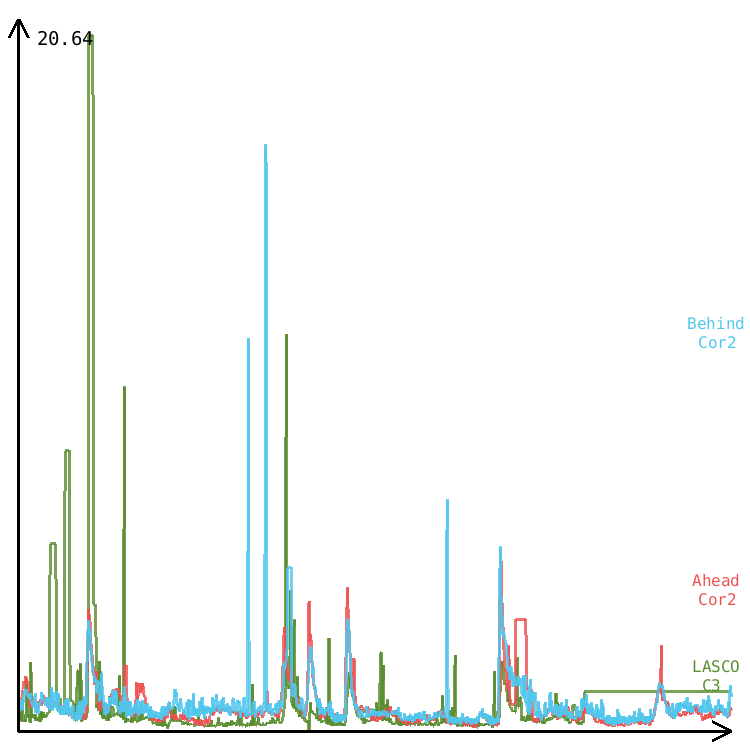
\includegraphics[width=\abSmallImageWidth]{figures/timelineview_soho_cor2.png}  
%  }
\subfigure {
  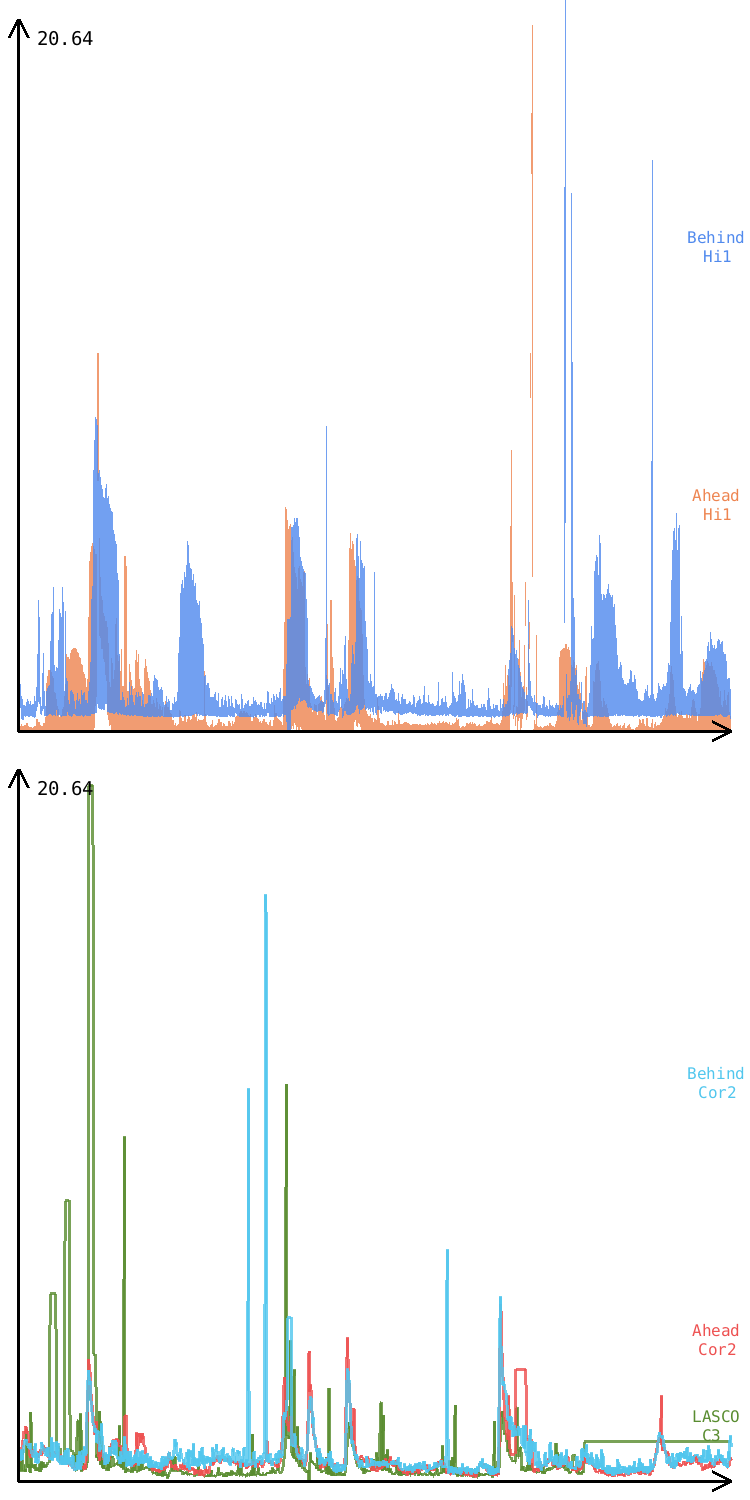
\includegraphics[height=\abImageHeight]{figures/timelineview_combined.png}
}
\caption{The Timeline view provides insight into the time-dependent comparison of measured velocities. For each instrument and satellite, the velocity of a passing CME is determined using optical flow analysis and compared against the extracted velocity from the simulation run. Here, the average speeds for each instrument (colored lines) is shown together with the measurements from the simulation (black lines). The numerical values are shown as an overlay. It is possible for the analyst to restrict the Timeline View to individual instruments (bottom right) and display the minimum and maximum velocities as line thickness (top right).}
\label{fig:timeline}
\end{figure*}

%\begin{figure*}
%\newcommand{\abImageWidth}{1.25\columnwidth}
%\newcommand{\abSmallImageWidth}{0.2\columnwidth}
%\centering
%\subfigure {
%  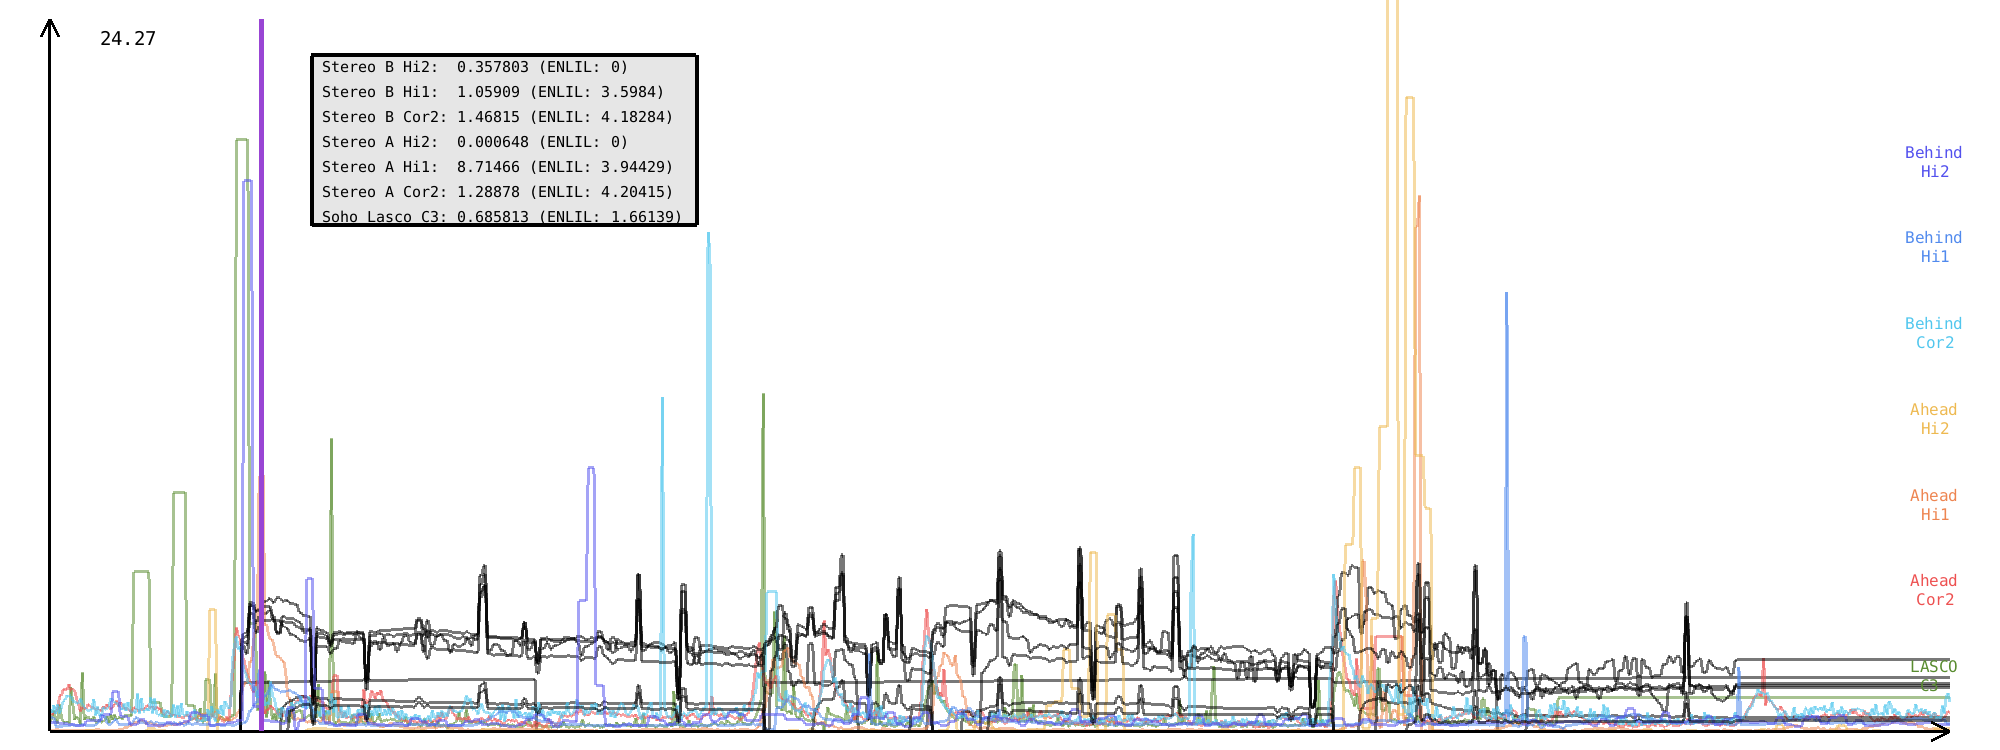
\includegraphics[width=\abImageWidth]{figures/timelineview_wide.png}
%}
%\begin{minipage}{0.3\columnwidth}
%  \subfigure {
%    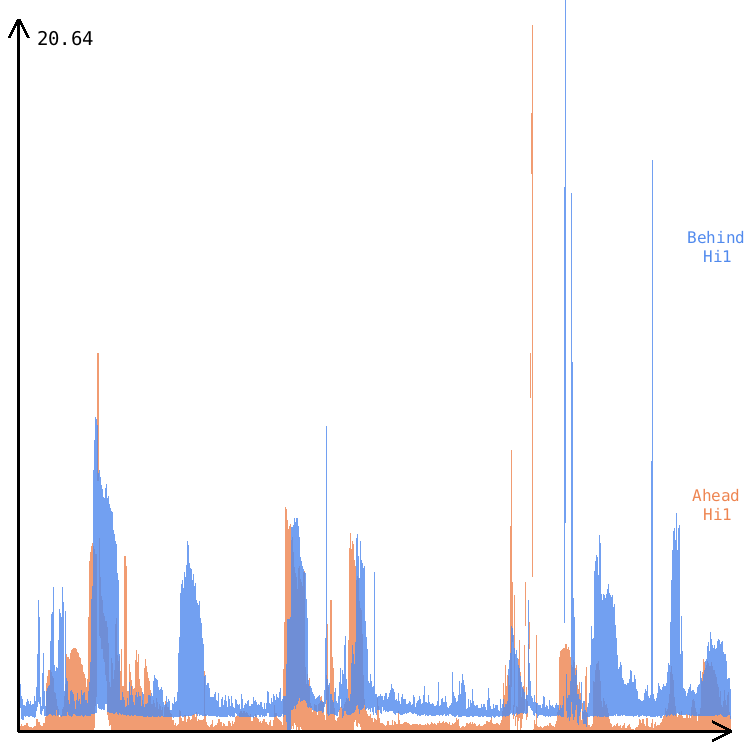
\includegraphics[width=\columnwidth]{figures/timelineview_hi1.png}
%  }
%
%  \subfigure {
%    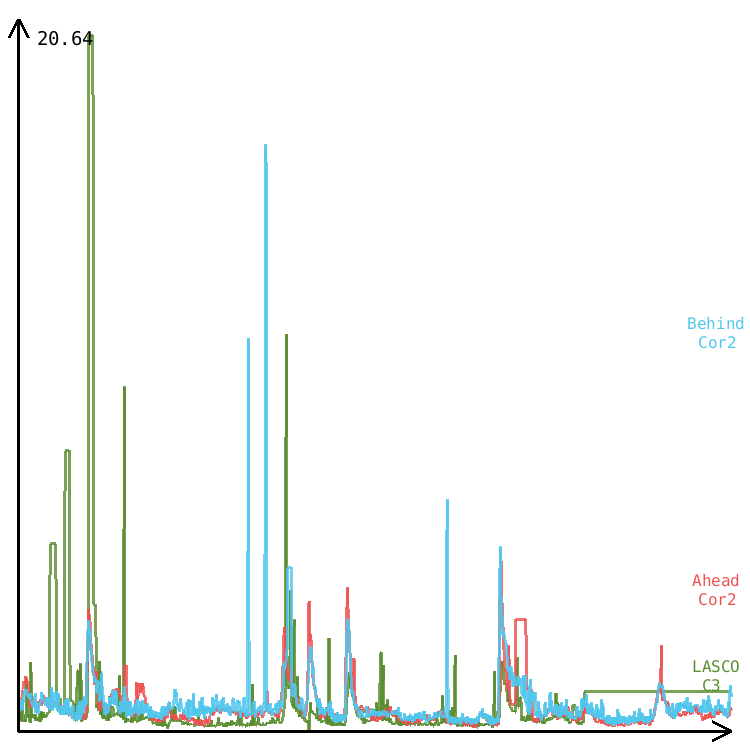
\includegraphics[width=\columnwidth]{figures/timelineview_soho_cor2.png}  
%  }
%\end{minipage}
%\caption{The Timeline view provides insight into the time-dependent comparison of measured velocities. For each instrument and satellite, the velocity of a passing CME is determined using optical flow analysis and compared against the extracted velocity from the simulation run. Here, the average speeds for each instrument (colored lines) is shown together with the measurements from the simulation (black lines).}
%\label{fig:timeline}
%\end{figure*}

The \emph{Ensemble Selection View} (see Figure~\ref{fig:selection}) provides an overview of all ensemble members and their validity as a glyph-based visualization. Each ensemble member is characterized by the 4 parameters: \emph{direction} (longitude and latitude), \emph{initial speed}, and the \emph{opening angle}. This view is separated into subviews to provide three cuts of this available 4 dimensional parameter space and designed in such a way to reflect the two dimensional projection of the cones onto the Sun's surface. To this end, the opening angle is mapped to the size of the circular glyph in all subviews. The main view shows the longitude and latitude on the horizontal and vertical axes, providing the direction of the cone when looking at the Sun. The longitude and latitude are normalized to the available parameter set to fill the available screen space. The side views show longitude and speed (bottom left) and speed and latitude (top right) on the horizontal and vertical axes respectively. This setup was chosen to provide a magic mirror-like effect, where glyphs from the main view can be projected in straight lines onto the side views to determine the respective velocities~\cite{konig1999multiple}. We investigated different setups, such as rendering cones in an interactive 3 dimensional environment or using different kinds of glyphs, but we chose this representation as it provided the most intuitive feedback to our experts.

The ground-truth measurements are compared against the predicted values from the ensemble members to retrieve a fitness value for each ensemble member. We chose the familiar red-green color scheme for the glyph to reflect how accurate the chosen prediction matches the measured data. The mapping from arrival time, speed and \kpIndex\ indices to color is normalized to the worst and best result respectively per simulation run. By doing this, we ensure that the view will always be useful to compare ensemble members, even if ensembles are of varying quality. There are three different variants for this view for the three in-situ measurements that we utilize; 1. the arrival time at an object, 2. the speed at which it arrives, and 3. the three \kpIndex\ indices that are calculated (see Section~\ref{sec:insitu}). We chose not to show three variants at the same time as the glyph would be otherwise cluttered with uncorrelated information. Instead, we allow the analyst to easily switch between the different variants to inspect the measurements. By providing the ability to switch between the variants without needing to look away from the screen, the analyst does not need to shift his focus away from the view and thus does not interrupt his workflow. Based on these measurements, the domain expert can make a pre-selection of valid ensemble members and focus his attention on border cases. The combination of an intuitive color scheme and location for each glyph enables the analyst to detect patterns and trends, such as a decrease in accuracy with a change in velocity, in the fitness of the ensemble, a possibility that is not available in the current workflow. These patterns can be used to start new simulation runs using new parameters for which the analyst expects better results, thus checking his hypotheses.

For the arrival time and the arrival speed, the entire glyph is of the same color. For the \kpIndex\ each glyph contains three fitness values, one for each predicted angle. In order to present the three predictions at the same time, and prepare the system to handle additional angles, we decided to divide the glyph into three segments, one for each angle prediction with the segments' locations reflecting the orientation of the predicted \kpIndex\ index (90\degree , 135\degree , and 180\degree ). To further increase the mental registration between segment location and angle orientation, we add an texture overlay to each segment that is rotated to reflect the angle prediction~(see Figure~\ref{fig:selectionkp}). The texture is represented by black lines that are oriented to agree with the angle of the \kpIndex\ for which they are used (90\degree\ horizontal, 135\degree\ angled, and 180\degree\ vertical respectively). Overlapping glyphs were not found to be a problem in the case of uniformly colored glyphs due to the clarity of each glyph. This is different for the \kpIndex\ indices due to an increased visual complexity and reduced contrast between different glyphs. In order to visually separate overlapping glyphs, we chose to add a thin black border that delineates each glyph in the view. In case of a total overlap of two glyphs in one view, they will always be separable in both subviews, as they have different velocities. Therefore, we do not require a mechanism to handle these situations.

In addition to the glyphs showing the ensemble members, we represent the median parameter set with an additional glyph that is marked with a cross. By adding the cross, we visually guide the analyst to the center of the view so that he intuitively knows where to start the analysis. Furthermore, the median glyph is rendered transparent to make it clear to the analyst that it is not a ensemble member that was generate by the parameter sweep.

Ensemble members can be selected by the user, which highlights the glyph in all subviews and provides numerical information about the member in the lower right corner. Furthermore, by selecting an ensemble member, its relevant data is loaded into the next view, the Timeline View, to be inspected in more detail in the next step of the workflow.

\subsection{Timeline View} \label{sec:timeline}
When an ensemble member is selected in the Ensemble Selection View, its timeline is presented in the \emph{Timeline View}~(see Figure~\ref{fig:timeline}). This view shows the CME's speed measured at all available time steps both for the coronagraph images as well as the simulation data. Displaying the speed was a reasonable choice for our experts as the accuracy of the speed has a direct correlation to the arrival time of a CME. At the same time, the CME's speed at each time step is an important measurement by itself as unexpected changes in velocity during the movement through interplanetary space often result in predictions errors and thus have to be investigated.

\subsubsection{Optical Flow Analysis} \label{sec:opticalflow}
The calibrated and preprocessed satellite images are publicly available on the Internet at the respective science teams' webpages\footnote{SOHO: http://sharpp.nrl.navy.mil/cgi-bin/swdbi/lasco/img\_short/form}\textsuperscript{,}\footnote{STEREO: http://stereo-ssc.nascom.nasa.gov/cgi-bin/images}. In order to extract the CME's velocity from the satellite images, we use optical flow analysis on subsequent pairs of images. Optical flow methods compute a vector field that describes the movement of features from one image to the next (see Figure~\ref{fig:opticalflow}). The optical flow method that we are using is the one presented by Sun~\etal\ that is one of the state-of-the-art optical flow implementations~\cite{sun2010secrets}. However, our system does not depend on the specific algorithm that is used to extract the optical flow. We found  that smoothing the images is a good compromise between the amount of detail and the signal-to-noise ratio.  It enhances the results as the satellite images are often the target of cosmic rays that have an effect on single pixels in the instruments' CCD chips. Thus, smoothing the image reduce the noise in the reconstructed velocity field. Using the optical flow analysis on the satellite images, we obtain the velocity direction and magnitude for each pixel projected onto the image plane. By taking the time between acquisition of images into account, we can thus compute the projected speed of the CME in each pixel for each image. Due to the location and geometric setup of the HI 1 and HI 2 coronagraphs (see Figure~\ref{fig:coronagraphgallery}), a passing CME must move to the left (STEREO A) or to the right (STEREO B). Therefore, we can discard velocity vectors that move in the opposite directions. These values are generated by background stars, the Milky Way, or planets as the satellites orbit around the Sun.

One source of inaccuracy in this technique that requires further study~(see Section~\ref{sec:futurework}) is the effect of Thomson scattering in the image. As we are dealing with a coronagraph in the visible spectrum of an optically thin plasma, the perceived brightness of the CME is dependent on the angle of the viewer and the light source---the Sun. This effect makes it difficult to measure densities based on image intensity and it is also known to distort the apparent location of the CME. However, Colaninno \etal\ found that using optical flow analysis for detecting velocities in CMEs could "provide quantitative measurements of the wave propagation speeds"~\cite{Colaninno:2006ef}.

\begin{figure}
\newcommand{\abSimulationImageWidth}{0.47\columnwidth}
\centering
\subfigure[Optical Flow Speed] {
  \fbox{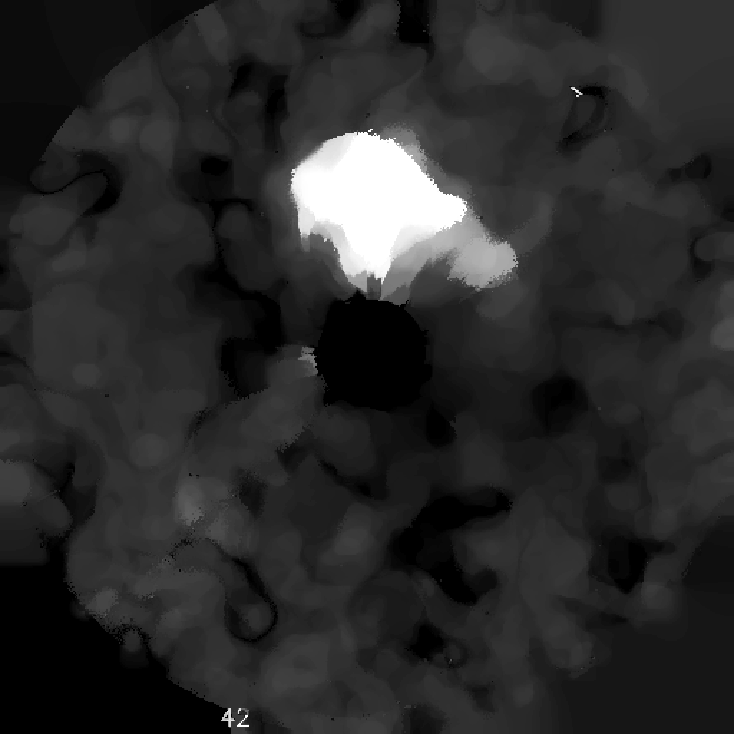
\includegraphics[width=\abSimulationImageWidth, height=\abSimulationImageWidth]{figures/20120713T094800.png}}
  \label{fig:opticalflow}
}
\hfill{}
\subfigure[Velocity gathering]{
  \fbox{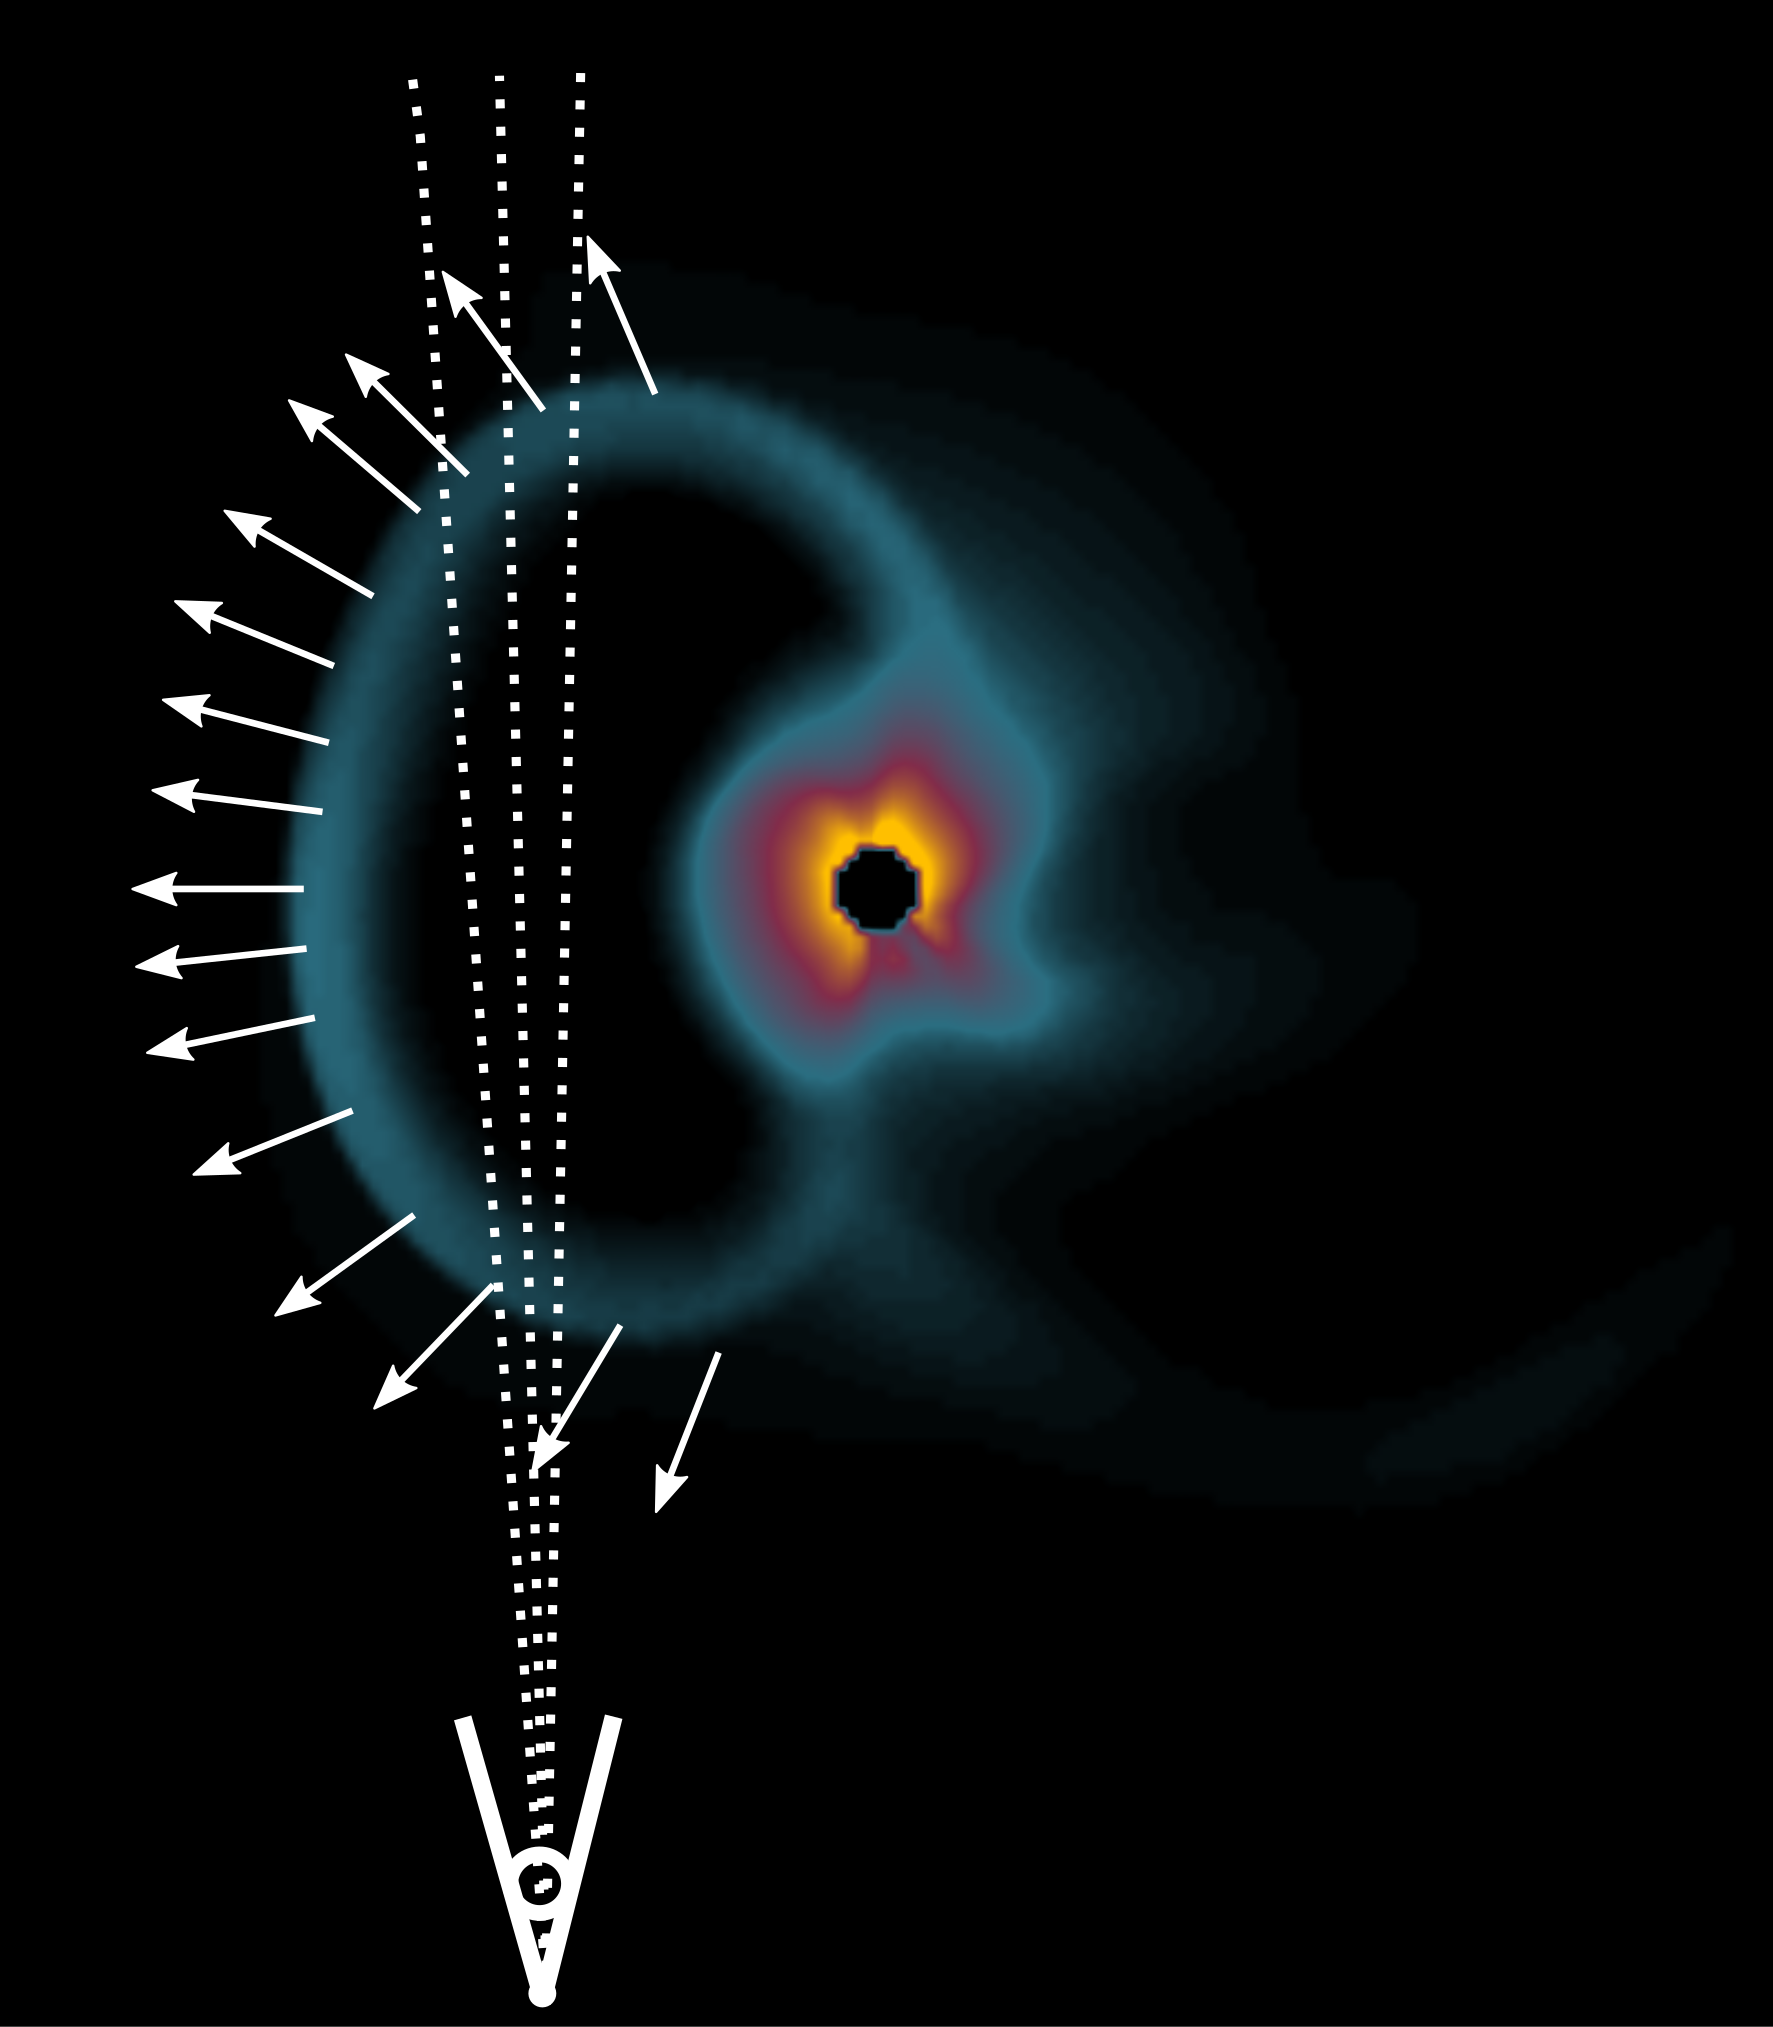
\includegraphics[width=\abSimulationImageWidth, height=\abSimulationImageWidth]{figures/cme_velocity.png}}
  \label{fig:simulationvelocitygathering}
}
\caption{(a) The magnitude of the screen-space speeds extracted using optical flow methods from the SOHO satellite at July 13 2012. (b) A schematic overview of the velocity distribution in a CME. By averaging all velocities along the view ray, every non-principal velocity vector is cancelled by the opposite side and only the principle velocity remains.}
\end{figure}

\subsubsection{Simulation Speed} \label{sec:simulationvelocity}
As the 3D velocity is one of the simulated parameters in the ENLIL MHD model, it is possible to directly extract it from the data. However, multiple aspects come into play in this approach. First, in order for a correct comparison, the scene camera has to be positioned at the correct location with the correct view direction and field-of-view settings. We retrieve those attributes from a library provided by NASA's Navigation and Ancillary Information Facility called SPICE\footnote{SPICE: http://naif.jpl.nasa.gov}. This allows for real-time accurate querying of satellite positions as well as the necessary instrument attributes. The second aspect becomes visible in Figure~\ref{fig:simulationvelocitygathering}; for each pixel in the image, there are many valid velocities in the dataset. To generate the resulting velocity vector for each pixel, we average the velocities for all samples along each view ray. As no further information about the CME is available, this approach provides the best approximation for the CME's velocity for each point.

In the ENLIL simulation the velocities are provided in spherical coordinates, as radial velocity and two angular velocities. We convert those velocities to Cartesian coordinates in order to project the simulation velocity vector into the image plane. This projection is necessary to be able to compare the simulation speed, given in world space coordinates, to the optical flow-based speed, given in screen-space coordinates. Given the image plane normal $n$ (which, in the case of a symmetric view frustum equal to the view direction) and a velocity vector $v$, we can retrieve the projected velocity vector $v_p = v\,-\,\left(\left(v \cdot n \right) * n \right))$. In a second step, we project $v_p$ into screen-space coordinates using the image size $s$, the field of view $f$ and the distance $d$ from the camera to the velocity: $ c = \left(s / f \right) \times \tan^{-1}\left( ||v_p|| / d \right)$. $c$ is the number of pixels that the projected velocity vector covers on the screen, thus being the same unit as returned by the optical flow method. For the distance $d$ we use the averaged world space position for each view ray for the distance calculation, analogous to the velocity. 

\subsubsection{Representation} \label{sec:representation}
We present the magnitude of both velocities to the user in a single graph view (see Figure~\ref{fig:timeline}). This allows the analyst to directly compare the two measured velocities for all instruments. The velocities are mapped to the vertical axis with time on the horizontal axis. In order to filter out any background velocities, we only consider values that lie above the 75\textsuperscript{th} percentile for each image. This approach was necessary as large parts of the image are filled with the background solar wind. Limiting the values to the 75\textsuperscript{th} percentile provided a useful value to filter the CME from the background, as the speed of the CME is orders of magnitude higher than the background solar wind. In order to suppress noise in the data, we apply a second filter to the data: as the initial speed is, with a level of uncertainty, known for each ensemble member, we have a lower limit to filter out values that can be attributed to errors in the optical flow algorithm. The value used for the centerline is the average of all velocities in an image after applying the filter. The analyst can change to view to also display the minimum and maximum values. The minimum and maximum values determine the thickness of the line at each time step and can be used by the analyst to judge the spread of velocities for each instrument (see Figure~\ref{fig:timeline} top right). In general, the analyst only needs the average speed, so the minimum and maximum values are not displayed constantly. By default the system presents all instruments to the expert at the same time, however we provide the possibility to only show individual instruments or satellites to allow for detailed inspection of individual measurements. This is especially relevant when inspecting minimum and maximum values, as the lines would otherwise overlap, creating visual clutter. In some cases it is necessary to exclude measurements, as the satellites are prone to image errors due to cosmic rays. 

The user can interact with the Timeline View using the mouse and inspect each individual time step. For each time, the values of the measured velocities are presented in an on-screen popup window. Furthermore, by selecting a specific time the analyst can load the related datasets in the third step of the workflow, the Spatial View, for in detail inspection.

%\todo{Continuous box plot}
%The information is grouped into three parts. First, the combined error for all satellites and instruments is shown. Second, the error is broken down for each satellite and shown as a stacked graph providing access to the individual error. Third, in the most detailed view the individual errors for the instruments are shown enabling detailed analysis of the potential sources of error in the simulation. For each mode, a selection follows the mouse and provides detailed information for each instrument at the selected time step. A stacked graph was chosen as it was shown that they are better suited for reading the overall trend~\cite{byron2008stacked}, a characteristic that is important for the overall error. The colors of the stacks have been selected to maintain a mental linking between instruments and their satellites. A primary color was chosen for each satellite, and perceptually similar colors are used for the corresponding instruments.

%The algorithm used for computing the time-varying error is deliberately held flexible. Currently, we are experimenting with an approach that uses optical flow analysis~\cite{sun2010secrets} and a perceptual difference metric~\cite{yee2004perceptual} to compare a rendering of the simulation data with the satellite imagery.



\subsection{Spatial View} \label{sec:rendering}
\begin{figure}
\newcommand{\abRenderingImageWidth}{\columnwidth}
\centering
\fbox{\includegraphics[width=\abRenderingImageWidth]{figures/renderingview.png}}
\caption{The Spatial View provides the analyst with access to all datasets we make use of in the system. It shows a volumetric rendering of the selected ensemble member at the given time. In the same scene, the images from the different satellites are integrated at their correct positions, giving the user the possibility to inspect the data.}
\label{fig:rendering}
\end{figure}

Selecting a time step in the Timeline View will set up the scene in the \emph{Spatial View} (see Figure~\ref{fig:rendering}). The rendered scene consists of the ENLIL simulation volume data, the spacecraft and planets at their correct positions, as well as the satellite images for the selected time step in their registered locations. As our collaborating space weather research center was not utilizing volume rendering to analyze the simulations before, there was a special interest to include this part in our system in order to be able to inspect the 3 dimensional structure of the CMEs. In the following steps, we will describe each individual component of the scene in detail.

\begin{figure}
\newcommand{\abSatelliteComparisonImageWidth}{0.4\columnwidth}
\centering
\subfigure {
  \fbox{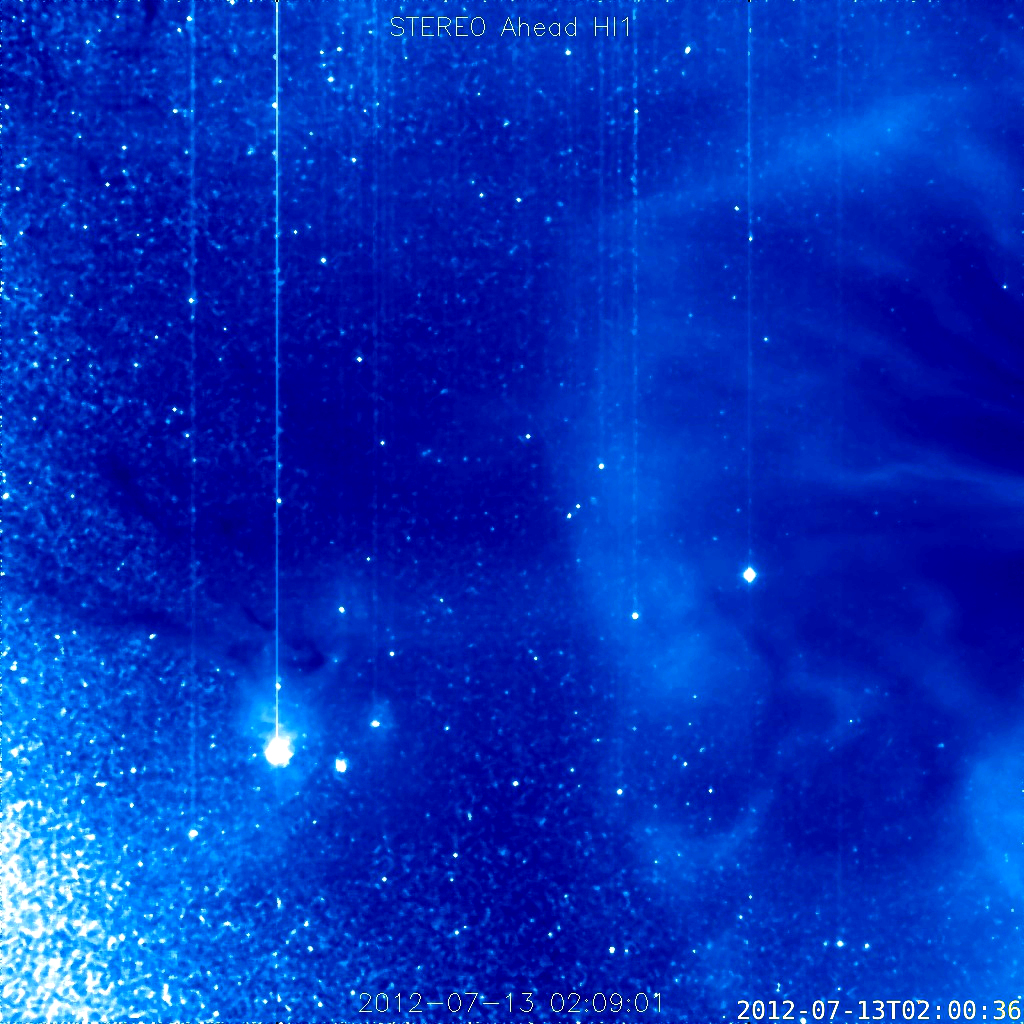
\includegraphics[width=\abSatelliteComparisonImageWidth]{figures/coronagraph.jpg}}
}
\subfigure {
  \fbox{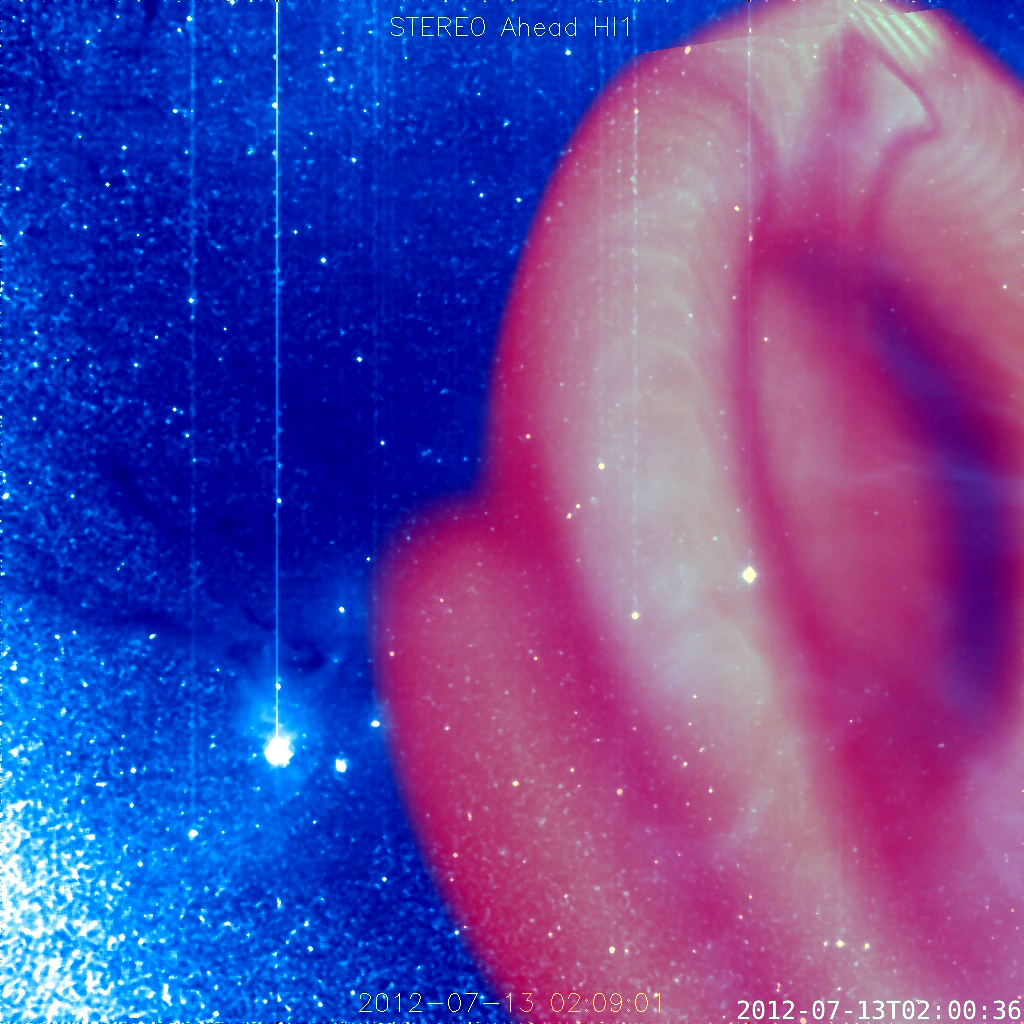
\includegraphics[width=\abSatelliteComparisonImageWidth]{figures/coronagraph_simulation.jpg}}
}
  \caption{Adding transparency allows the user to quickly compare the results of the simulation's volume rendering with the available coronagraph images.}
\label{fig:satellitecomparison}
\end{figure}

\subsubsection{Satellite Images} \label{sec:satelltes}
Providing the expert with the ability to inspect the satellite data together with the other modalities is crucial, as the analyst can directly compare the satellite images with the simulation data and thus gain additional insight about the level of agreement between simulation and satellite images. By locating the differences in the timeline view and investigating them in detail, we help the analyst understand the reasons for the discrepancy. In order to ease these comparisons, we provide an interface to the user to quickly and accurately move the camera into the location of a satellite with the correct orientation and field of view, as well as interactively modify the transparency of all image projections (see Figure~\ref{fig:satellitecomparison}).

For each satellite and each instrument the most accurate image, i.e. the image that is least out of date, is projected onto a plane in the scene using perspective texturing as described by Everitt~\etal~\cite{Everitt:2001tg}. The location and attributes of the virtual camera is retrieved using NAIF's SPICE library in the same way as done for the velocity images. The distance of the virtual image plane to the camera can be modified by the user and the image is correctly placed in the field of view of the instrument. The image data, alongside its metadata, is retrieved from the FITS files that are published by the respective science teams~\cite{wells1981fits}. These files include information about exposure, acquisition time, internal roll angle of the spacecraft and more. The combination of the SPICE information and the FITS information provides the rendering with all information necessary coregister the coronagraph images.

\subsubsection{Volume Rendering} \label{sec:volumerendering}
The ENLIL MHD simulation code in our system is natively computed on a spherical grid with the Sun in the origin. This means that the data is available as a rectangular volume where the principal axes are the radius $r$, longitude $\phi$, and latitude $\theta$. Instead of resampling the volume onto a regular grid, which would drastically increase the memory requirements, we perform a modified version of the raycasting scheme introduced by Kr\"uger and Westermann~\cite{Kruger:2003ge} that performs the raymarching in Cartesian world space, but transforms each sample point into the spherical sample space. This method was inspired by the work of Balabanian~\etal , who applied a similar technique for the visualization of fish schools~\cite{balabanian-2007-ant}.

Instead of a cubic proxy geometry, we utilize a tessellated sphere as the entry-exit points. In the case of spherical geometry, this provides the rendering with an effective  and inexpensive empty space skipping since about 50\% of the otherwise empty volume is removed. During the raymarching, each Cartesian prospective sampling point $(x,y,z)$ on the view ray is transformed into the spherical coordinate system and the resulting tuple $(r, \phi, \theta)$ is used to look up the value in the spherical volume.

\begin{figure}[b!]
\newcommand{\abImageWidth}{0.65\columnwidth}
\centering
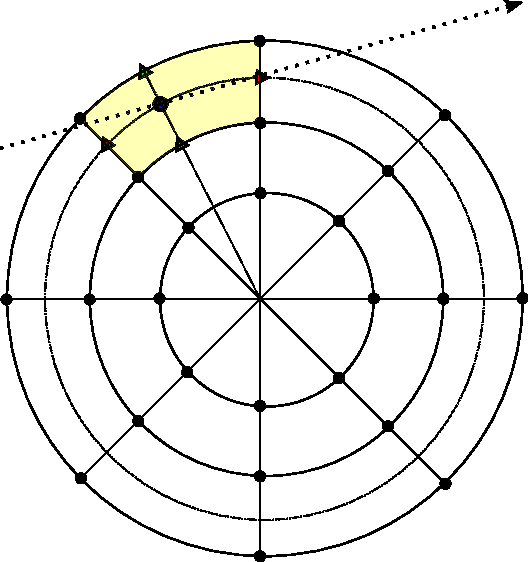
\includegraphics[width=\abImageWidth]{figures/spherical_interpolation.pdf}
\caption{A representation of the interpolation scheme that we employ on the spherical data. In the example we want to retrieve the value at the blue sampling location. While the (linear) radial interpolation provides the green values, the interpolation in $\phi$ takes into account the red values.}
\label{fig:sphericalvolume}
\end{figure}

\begin{figure}
\newcommand{\abImageWidth}{0.45\columnwidth}
\centering
\fbox{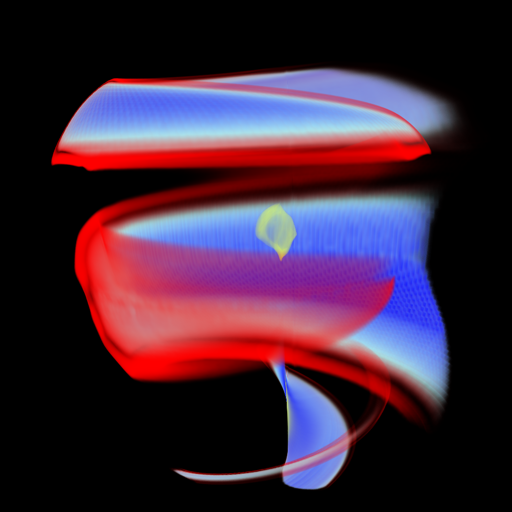
\includegraphics[width=\abImageWidth]{figures/performance_adaptive_no.png}}
\fbox{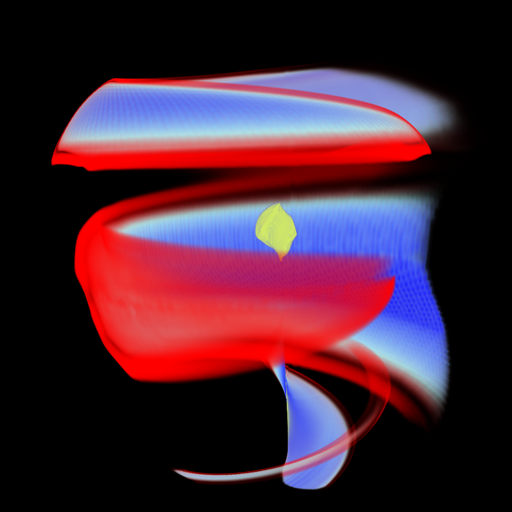
\includegraphics[width=\abImageWidth]{figures/performance_adaptive_05_05.png}}
\caption{Comparison images between regular sampling (a) and adaptive sampling (b) showing increased sampling density close to the center where data density is higher.}
\label{fig:sphericaladaptivesampling}
\end{figure}


\noindent {\bfseries Interpolation.} For each sample point along the ray, trilinear interpolation is performed along the $r$, $\phi$, and $\theta$ axes (see Figure~\ref{fig:sphericalvolume}). Using this scheme, the interpolation is effectively performed along great circles in the volume and thus performs analogous to Spherical Linear Interpolation (SLERP). We investigated the difference between positional interpolation that is based on the Cartesian position, and the above mentioned value interpolation that is performed in the spherical sample space. In our experiments, we found a slightly improved result through the value interpolation at negligible performance cost.

\noindent {\bfseries Adaptive sampling.} An additional benefit of the spherical volume is the distribution of sample points. While it is a regular distribution in spherical sample space, when converting samples into Cartesian world space, it becomes non-uniform with a density fall-off of $1/r^3$ (see Figure~\ref{fig:sphericalvolume}). It is possible to exploit the $1/r^3$ dependency in data density in the rendering step to perform data-aware importance sampling along the view ray. As the data density decreases in the outer areas of the sphere, it is sufficient to coarsen the sampling of the view ray. Likewise, it is beneficial to decrease the sampling step size closer to the origin where the data density increases. This technique is not limited to a spherical volume, but it is trivially integrated as the radial distance to the center is already available for each sample point. Using this technique, we achieved improved visual quality while, at the same time, increasing the rendering performance by a factor of 2 (see Figure~\ref{fig:sphericaladaptivesampling}).

\noindent {\bfseries Variables.} The ENLIL simulation code produces multi-variate datasets for each ensemble member. Of the 29 available variables, we utilize 3 in this part of our system. 1. the $N \cdot r^2$ variable denotes the number of particles that are present in the space covered by each voxel. The multiplication by $r^2$ negates the radial density falloff and allows us to utilize a single transfer function for the entire volume. 2. the $\rho$ parameter is the density of particles. We perform multi-volume rendering using both parameters for our final results in order to visually separate the background solar wind and the different structures within the CME. Together with the analysts, we devised a method to improve the simulation output's use for volume rendering. Instead of running the simulation once, ENLIL now produces the CME-infused variables as before, but also computes a second set of variables only containing the background solar wind, without the CME. We display the difference between the two simulation runs, resulting in a more accurate rendering of the CME structure, making the volume rendering easier to comprehend. We could perform the same operation for the velocity field as computed in Section~\ref{sec:simulationvelocity}, but the speed of the background solar wind is orders of magnitude lower than the speed of the CME, thus the effect of this subtraction would be minimal. 3. the $dp$ parameter is a set of tracer particles that are spawned in the original cone that described the CME's direction, speed, and opening angle. By advecting and tracing these particles between time steps, it is possible to use this parameter as a segmentation mask for the CME in the volume rendering. In rendering, each sample point first samples the $dp$ volume which is used as a segmentation volume, modified by a transfer function. Then, the other volumes are only sampled if the $dp$ transfer function response is positive.

\subsubsection{Integrated Rendering} \label{sec:integration}
The ability to combine multiple volumes with transparent geometry is necessary to allow the space weather analyst to compare the satellite images with the results of the volume rendering in the same setup by fading the satellite images. Furthermore, the 3 dimensional volume rendering is the first time that the full structure of the CME is considered in the analysts workflow.

In order to display the volume rendering coregistered with multiple transparent geometries, we make use of an order-independent transparency method. Our system uses a per-fragment sorting technique that is based on an A-Buffer technique as presented by Lindholm~\etal~\cite{Lindholm:2014fm}. The technique operates by gathering fragments in a per-pixel linked list that is depth sorted in a second pass, thus allowing for high-performant support of a sufficient level of depth complexity and the possibility of transparent objects integrated within the volume rendering. 

\section{Application Case} \label{sec:applicationcase}
We applied our system to multiple application cases, such as the Carrington-level CME of July 2012~\cite{baker2013major} or a simulation run of a CME from May 2011. However, the main application case for this paper is the real-time ensemble modeling of an Earth-directed CME that was observed on 18 April 2014. This CME was associated with an M7.3 class solar flare from Active Region 12036 located at S18\degree W29\degree with a peak at 13:03 UT. For more detailed information about the CME and description of the manual ensemble generation process, we refer the reader to~\cite{mays2015ensemble}. The application case consists of 36 ensemble members with the CME propagation directions clustered between -30\degree\ to -40\degree\ latitude, and around 10\degree\ west of the Sun-Earth line in longitude, while CME speeds range from $\approx$1300 to 1600 km/s. The median CME parameters are: speed of 1394\,km/s, direction of 9\degree\ longitude, -35\degree\ latitude, and a half-width of 46\degree . The prediction error for the mean predicted CME arrival time was -5.2 hours and the observed arrival time was just within the ensemble predicted spread. The ensemble members with arrival times closest to the observed time had CME input speeds in the range of 1200-1400 km/s, latitudes near -40\degree\ and half widths around 35\degree -40\degree . The NOAA real-time observed \kpIndex\ index reached 5 on 20 April with the CME arrival. The standard deviation of the overall \kpIndex\ forecast probability distribution is 1.1, with 84\% of the forecasts falling between \kpIndex\ 5 to 7.

Figure~\ref{fig:selection} shows the Ensemble Selection view for this event. In the main view, it shows that ensembles with lower latitudes and lower speeds were more accurate in predicting the arrival time. Retrieving this information from the ensemble member was not possible before in the old workflow, as the connection between accuracy and direction was not presented. This information can now be used to query new simulations with low latitude and low speed to find the best agreement with the ground truth data. Figure~\ref{fig:selectionkp} shows the comparisons of geoeffectivities for the same event. It shows immediately that the 90\degree\ magnetic field clock angle agrees is the most accurate prediction, followed by the 135\degree\ angle. Even if this information is also available in the plots, the glyph based representation shows this information more clearly to the analyst.

Using the volumetric rendering, our experts have gained new insight into the 3 dimensional structure of the CME. They found holes in the shock front of the CME, which were previously unknown and will result in a solar physics publication (see Figure~\ref{fig:cmestructure}). Furthermore, it is used for ruling out unphysical simulation results. For example in a magnetosphere simulation, plasma was ejected against the solar wind flow direction from the dayside Earth's magnetosphere and high-velocity flows were found in the inner magnetosphere. These features have not been observed and the model was modified to provide a more numerically stable coupling between the magnetosphere and the inner magnetosphere ring current modeling component using a different set of kinetic physics equations.

\section{Conclusions \& Future Work} \label{sec:futurework}
\begin{figure}
\newcommand{\abImageWidth}{0.45\columnwidth}
\centering
\subfigure {
  \fbox{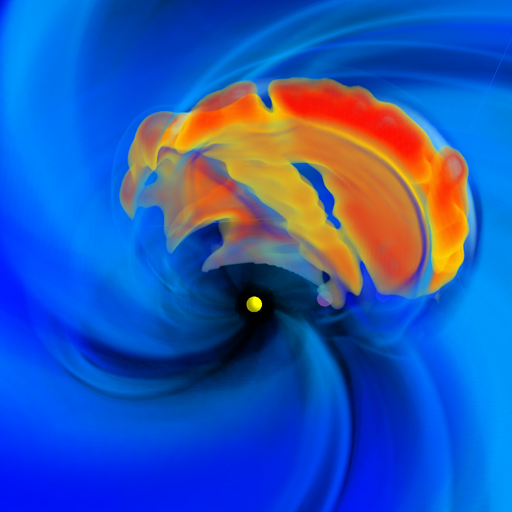
\includegraphics[width=\abImageWidth]{figures/cme_structure.png}}
}
\subfigure {
  \fbox{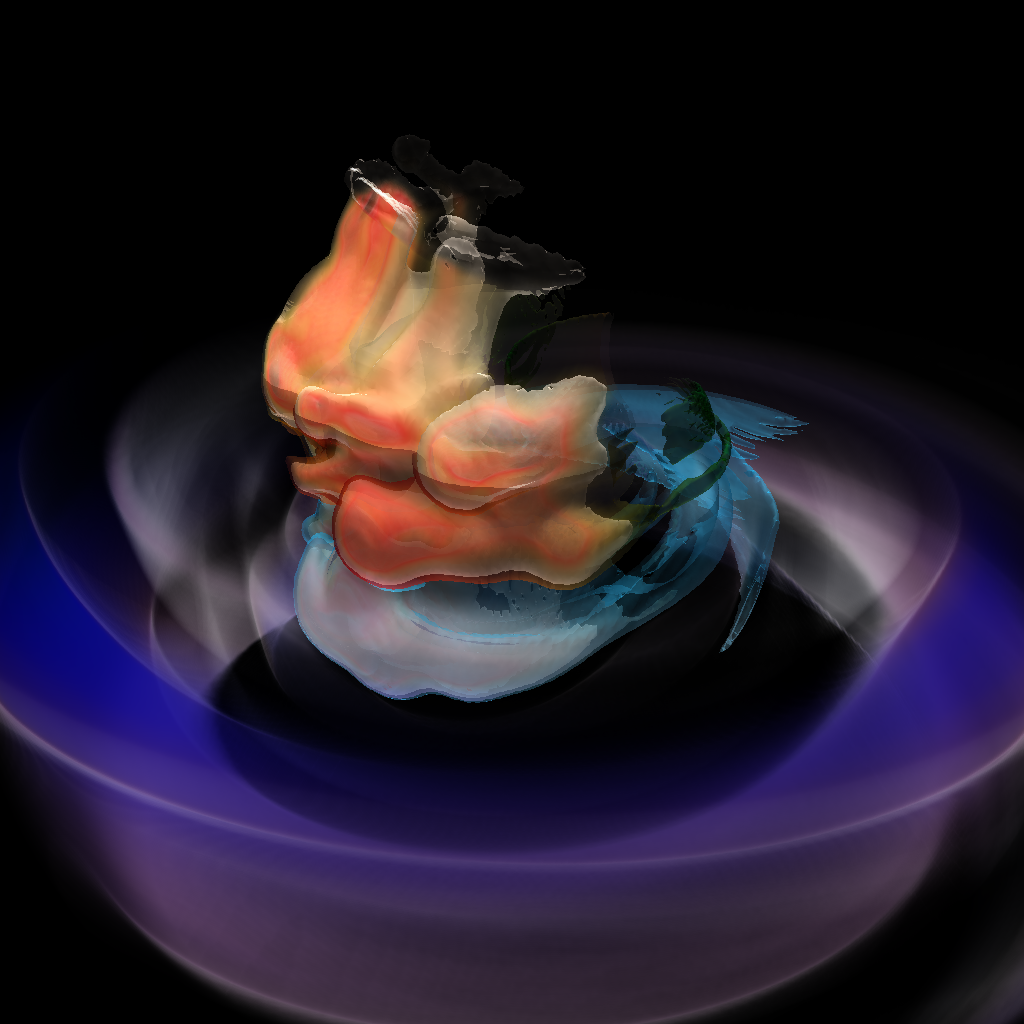
\includegraphics[width=\abImageWidth]{figures/space.png}}
}
\caption{Two CME structures contained in the simulation datasets that were discovered using our system and were previously not known to exist to the space weather analysts.}
\label{fig:cmestructure}
\end{figure}


In this paper, we proposed a system that enables space weather analysts to explore the parameter space of ensemble simulations of coronal mass ejections. The system was developed in close collaboration with leading expert analysts from one of the few space weather research centers in the world in a participatory design approach. This approach proved to be successful due to the rapid iterations in the development process and has been beneficial for both the visualization aspects as well as the space weather research aspects of the project.

We presented a visualization system using a three-tier workflow that allows the analyst to compare ensemble simulations with measured in-situ data, to correlate the time-dependent evolution of interplanetary coronal mass ejections with optical flow analysis from satellite images, and to inspect a 3D volumetric rendering of the simulation dataset with integrated satellite images and spacecraft positions. Using our system, the analyst can gain a deeper understanding of the parameter sensitivity of ensemble simulations and, at the same time, inspect the CME's 3 dimensional structure for each ensemble member.s

For future work, we would like to further improve the usability of the system based on the inspiration of the domain experts. Instead of relying on averaging for retrieving the velocity field from the simulation data, we want to investigate reconstruction approaches that are based on the density distribution in the CME. In order to achieve this and, in the process, make the output of the volume rendering more comparable to the coronagraph images, we will implement multiple scattering techniques into our system in order to physically accurately simulate Thomson scattering~\cite{howard2012thomson} and create synthetic coronagraph images. As a measure to improve the quality of the optical flow algorithm, we want to design an optical flow algorithm that takes the unique, radial-dominant aspects of the coronagraph images into account. Lastly, we will investigate the use of interplanetary scintillation as another, real time, measurement with which to compare the simulated coronal mass ejection.

%% if specified like this the section will be committed in review mode
\section*{Acknowledgments}
The presented visualization concepts have been realized using the Voreen framework (www.voreen.org). Simulation results have been provided by the Community Coordinated Modeling Center at Goddard Space Flight Center through their public Runs on Request system (http://ccmc.gsfc.nasa.gov). The CCMC is a multi-agency partnership between NASA, AFMC, AFOSR, AFRL, AFWA, NOAA, NSF and ONR.
%\nocite{*}
%\newpage

\bibliographystyle{abbrv}
%%use following if all content of bibtex file should be shown
%\nocite{*}
\bibliography{bibliography}
\end{document}

